%==============================================================================
% Masters Thesis Document
% This document template is adapted by Lester James V. Miranda
% for his Masters thesis in Waseda University.
%
% Using LaTeX Template Version 2.5 (27/8/17)
% The template was downloaded from:
% http://www.LaTeXTemplates.com
%
% Version 2.x major modifications by:
% Vel (vel@latextemplates.com)
%
% This template is based on a template by:
% Steve Gunn (users.ecs.soton.ac.uk/srg/softwaretools/document/templates/)
% Sunil Patel (sunilpatel.co.uk/thesis-template/)
%
% This file is part of thesis-manuscript.
%
% thesis-mansucript is free software: you can redistribute it and/or modify
% it under the terms of the GNU General Public License as published by
% the Free Software Foundation, either version 3 of the License, or
% (at your option) any later version.
%
% thesis-manuscript is distributed in the hope that it will be useful,
% but WITHOUT ANY WARRANTY; without even the implied warranty of
% MERCHANTABILITY or FITNESS FOR A PARTICULAR PURPOSE.  See the
% GNU General Public License for more details.
%
% You should have received a copy of the GNU General Public License
% along with thesis-manuscript.  If not, see <http://www.gnu.org/licenses/>.
%
%==============================================================================

%------------------------------------------------------------------------------
%	PACKAGES AND OTHER DOCUMENT CONFIGURATIONS
%------------------------------------------------------------------------------

\documentclass[11pt,
            english,
            oneside,
            liststotoc,
            singlespacing,
            headsepline,
            consistentlayout]{style}
\usepackage[utf8]{inputenc}
\usepackage[T1]{fontenc}
\usepackage{mathptmx}
\usepackage[backend=biber,style=authoryear,natbib=true]{biblatex}
\usepackage[autostyle=true]{csquotes}
\usepackage{enumitem}
\usepackage{amsmath}
\usepackage{wrapfig}
\usepackage{algorithm}
\usepackage{algpseudocode}
\usepackage{threeparttable}
\usepackage{footmisc}


\addbibresource{bibliography.bib}

\listfiles


%------------------------------------------------------------------------------
%	OTHER SETTINGS
%------------------------------------------------------------------------------
\setcounter{tocdepth}{1}
\setitemize{itemsep=1pt}        % Modify spacing between items
\renewcommand{\arraystretch}{1.2} % Stretch tables

% Command for algorithm INPUT and OUTPUT
\algnewcommand\algorithmicinput{\textbf{Input:}}
\algnewcommand\INPUT{\item[\algorithmicinput]}
\algnewcommand\algorithmicoutput{\textbf{Output:}}
\algnewcommand\OUTPUT{\item[\algorithmicoutput]}

% Set-up footnotes
\renewcommand{\thefootnote}{\fnsymbol{footnote}}



%------------------------------------------------------------------------------
%	MARGIN SETTINGS
%------------------------------------------------------------------------------

\geometry{
    paper=letterpaper, % Change to letterpaper for US letter
    %inner=2.5cm, % Inner margin
    %outer=3.8cm, % Outer margin
    %bindingoffset=.5cm, % Binding offset
    top=1.5cm, % Top margin
    bottom=1.5cm, % Bottom margin
    %showframe, % Uncomment to show how the type block is set on the page
}

%------------------------------------------------------------------------------
%	THESIS INFORMATION
%------------------------------------------------------------------------------

\thesistitle{
    Predicting Protein Functions via Selective Feature Extraction
    using a Mutually-Competitive Autoencoder
}
\supervisor{Dr. Jinglu Hu}
\degree{Master of Engineering}
\author{Lester James V. Miranda}
\addresses{}

\subject{Masters Thesis of Lester James V. Miranda}
\keywords{
    machine learning,
    bioinformatics,
    feature extraction,
    multi-label classification
}
\university{Waseda University}
\department{Graduate School of Information, Production, and Systems}
\group{Furuzuki Neurocomputing Systems Laboratory}
\faculty{Information Architecture}

\AtBeginDocument{
\hypersetup{pdftitle=\ttitle}
\hypersetup{pdfauthor=\authorname}
\hypersetup{pdfcreator=\authorname}
\hypersetup{pdfproducer=\authorname}
\hypersetup{pdfkeywords=\keywordnames}
\hypersetup{pdfsubject=\subject}
}

\begin{document}

\frontmatter

\pagestyle{plain}

%------------------------------------------------------------------------------
%	TITLE PAGE
%------------------------------------------------------------------------------

\begin{titlepage}
\begin{center}
\vspace*{.02\textheight}
{\LARGE \bfseries \ttitle}\vspace{2.5cm} % Thesis title

{\Large 44161652-3: \authorname} % Author name
\vfill 

{\normalsize \degreename} \\[2.5cm] % Degree

{\normalsize Supervisor: \supname} \\[2.5cm] % Supervisor's name

{\normalsize \groupname} \\        % Laboratory affilation
{\normalsize \facname}   \\        % Faculty affiliation
{\normalsize \deptname}  \\[0.5cm] % Departmental affiliation

{\normalsize \univname} \\[0.5cm] % University affiliation

{\normalsize \today} % Current date
\end{center}
\end{titlepage}

%------------------------------------------------------------------------------
%	SECOND TITLE PAGE
%------------------------------------------------------------------------------
\begin{titlepage}
\begin{center}
\thispagestyle{empty}
\vspace*{.02\textheight}
{\ttitle} \\[2.5cm] % Thesis title
{44161652-3: \authorname} \\[2.5cm] % Author name
{
    A thesis submitted to the Graduate School of \\
    Information, Production, and Systems\\
    Waseda University\\
    in partial fulfillment of the requirements for the degree of
} \\[1.2cm]

{\degreename} \\[2.5cm]
{Supervisor: \supname} \vfill

{\deptname}\\[1.0cm]
{\univname}\\[1.0cm]
{\today} \vfill

{Copyright \textcopyright 2018 44161652-3: \authorname} \\[0.2cm]
All Rights Reserved
\end{center}
\end{titlepage}


%------------------------------------------------------------------------------
%	ABSTRACT PAGE
%------------------------------------------------------------------------------

\begin{abstract}
\addchaptertocentry{\abstractname} % Add the abstract to the table of contents


\vfill
\noindent \textbf{Keywords}\textemdash\keywordnames
\end{abstract}

%------------------------------------------------------------------------------
%	ACKNOWLEDGEMENTS
%------------------------------------------------------------------------------

\begin{acknowledgements}
\addchaptertocentry{\acknowledgementname} % Add the acknowledgements to the table of contents

\end{acknowledgements}

%------------------------------------------------------------------------------
%	LIST OF CONTENTS/FIGURES/TABLES PAGES
%------------------------------------------------------------------------------

{
\hypersetup{linkcolor=black}
\tableofcontents % Prints the main table of contents
\listoffigures % Prints the list of figures
\listoftables % Prints the list of tables
}
%------------------------------------------------------------------------------
%	SYMBOLS
%------------------------------------------------------------------------------

\begin{symbols}{lll} % Include a list of Symbols (a three column table)



\addlinespace % Gap to separate the Roman symbols from the Greek

$\omega$ & angular frequency & test \\

\end{symbols}


%------------------------------------------------------------------------------
%	THESIS CONTENT - CHAPTERS
%------------------------------------------------------------------------------

\mainmatter % Begin numeric (1,2,3...) page numbering

\pagestyle{thesis} % Return the page headers back to the "thesis" style

%=============================================================================
% Introduction
% Copyright (c) 2018. Lester James V. Miranda
%
% This file is part of thesis-manuscript.
%
% thesis-mansucript is free software: you can redistribute it and/or modify
% it under the terms of the GNU General Public License as published by
% the Free Software Foundation, either version 3 of the License, or
% (at your option) any later version.
%
% thesis-manuscript is distributed in the hope that it will be useful,
% but WITHOUT ANY WARRANTY; without even the implied warranty of
% MERCHANTABILITY or FITNESS FOR A PARTICULAR PURPOSE.  See the
% GNU General Public License for more details.
%
% You should have received a copy of the GNU General Public License
% along with thesis-manuscript.  If not, see <http://www.gnu.org/licenses/>.
%
% Created by: Lester James V. Miranda <ljvmiranda@gmail.com>
%=============================================================================

\chapter{Introduction}
\label{Introduction}

\par In bioinformatics, predicting a protein's function is a fundamental task.
If a protein's functional category is known, then designing drugs or
identifying a disease's molecular mechanism is achievable. However, acquiring
this knowledge is slow and difficult due to the complexity in a protein's
biological information, and the unfamiliarity of life's organization at the
molecular level (\cite{baldi2001bioinformatics}). In addition, more and more
proteins are being characterized by high-throughput sequencing techniques
today, creating vast stores of genomic data available for use
(\cite{gaudet2017gene, cozzetto2017computational}). This widens the gap between
annotated and unannotated proteins, urging the need for a more efficient,
accurate, and fast set of prediction techniques in the presence of
``genomic big data.''

\par Machine learning techniques have been observed to perform well in complex
tasks involving large amounts of data (\cite{chen2014data}). They have been
exceptional in recognizing patterns and learning from a vast number of examples 
(\cite{lecun2015deep}). Before prediction, a machine learning model must first
discern a pattern from a set of data, and use that to infer the category, or 
\textit{class}, a new sample belongs to. Because most proteins can perform
multiple functions at once, \textit{multi-label classification}\textemdash
a subset of machine learning\textemdash is used. However, the effectiveness of
a multi-label classification model still depends on the pattern it learns, and
how well it represents the input data provided.

\par Learning to understand data and representing it in a form beneficial for a
machine learning model is known as \textit{representation learning}. Although
it is entirely possible to manually engineer characteristics, or \textit{features}
, of a dataset, it is labor-intensive and requires thorough domain-expertise 
(\cite{bengio2013representation}).  Instead, it is preferable to automatically
extract useful information from data using a \textit{feature extractor}, and
ensure that the new features are relevant. Selecting more relevant features is
apt for protein datasets because it is noisy, i.e., both relevant and irrelevant
data are present. Properly discerning which characteristics are important and 
transforming them into features useful to a predictor is essential in
identifying protein functions.

\par This research presents a novel architecture based on the autoencoder neural
network. The proposed network motivates selective behavior in order to produce
relevant features. This is done through mutual competition: adjusting the
backpropagation path to keep a select number of neurons active while ensuring
meaningful representations. It is expected that this method will be able to
predict protein functions well, as compared to using raw data directly or to
other techniques in literature. 

\newpage

\par \noindent The rest of the document is organized as follows:

\begin{itemize} 
    \item The remaining sections of Chapter \ref{Introduction}
        discuss the context behind this work (Sec. \ref{Background}), the
        research motivation (Sec. \ref{Motivation}), and the formulation of the
        research problem (Sec. \ref{Problem}).  
    \item Chapter \ref{LiteratureReview} comments on the related literature
        that also tackles the problem of protein function prediction. 
    \item Chapter \ref{Methodology} outlines the proposed method
        and gives an overview of its training and testing schemes (Sec. 
        \ref{Overview}). In addition, an explanation of the datasets used (Sec.
        \ref{Datasets}) and a description of the experimental environment
        (Sec. \ref{ExperimentalEnvironment}) will be done. 
    \item Chapter \ref{Results} discusses the experiments conducted to evaluate the 
        proposed method: benchmarking performance with other techniques 
        (Sec. \ref{Benchmarking}), measuring model quality (Sec.\ref{ModelQuality}),
        and estimating feature relevance (Sec.\ref{FeatureRelevance}).
    \item Lastly, Chapter \ref{Conclusion} concludes the work. Potential avenues for 
        future research (Sec. \ref{FutureWork}) will be discussed.
\end{itemize}


\section{Background of the Study}
\label{Background}

Approaching the problem of protein function prediction requires the
understanding of how protein data is represented. Proteins are always
described into two: first by their (1) \textbf{features} or characteristics,
and second by their (2) \textbf{labels} or set of functions it performs. This
section will discuss these types of data, and give a brief background on two
related topics: \textbf{multi-label classification}, a set of machine learning
methods for predicting multiple associations in a sample, and \textbf{feature 
extraction}, a technique for finding new representations from raw data.

\subsection{Protein features}

\par Proteins can be described into either sequences or expressions 
(\cite{xiong2006essential}). Sequences describe the protein as a chain
of amino acids, the building blocks of protein, represented by a single letter.
When arranged into a sequence, the order of appearance becomes important.
On the other hand, expressions describe the protein as combinations of various
techniques such as micro-array expression data, phylogenetic profiles and DNA
chips. It represents proteins as a vector of numerical values containing the
output of the micro-array process.

\par Although prediction is possible using protein sequences
(\cite{whisstock2003prediction, devos2000practical}), expressions have
been observed to be effective in predicting protein functions
(\cite{eisenberg2000protein, marcotte1999combined}). Thus, this
research will focus on the latter as descriptors for protein data. In
particular, micro-array expression data and phylogenetic profiles will
be used (See Sec. \ref{Datasets})

\subsection{Protein functions}

\par Proteins can belong to one or more functional categories. They
refer to various life processes such as metabolism, cell
reproduction, synthesis that arranged in an ontology. This
organization enables researchers to observe the relationships and 
properties of protein functions, and is one of the standard tools
in bioinformatics today.

\par Various ontologies describe a protein's functional category,
and two of the most common are the Gene Ontology (GO) and the Munich
Information Center for Protein Sequences (MIPS) annotations
(\cite{gaudet2017gene, mewes2006mips}). Although each differ on their
experimental methods, they remain similar by representing
protein functions as a direct acyclic graph (DAG) to express the relationship
between its members (e.g., ``is-a'', ``part-of'', etc.). To illustrate,
Figure \ref{demo:yeast_go} shows the gene ontology of the  function ``cellular
bud site selection'' performed by YAL041W, a protein found in
\textit{S. cerevisiae} or baker's yeast.

\begin{figure}[!t]
  \centering
  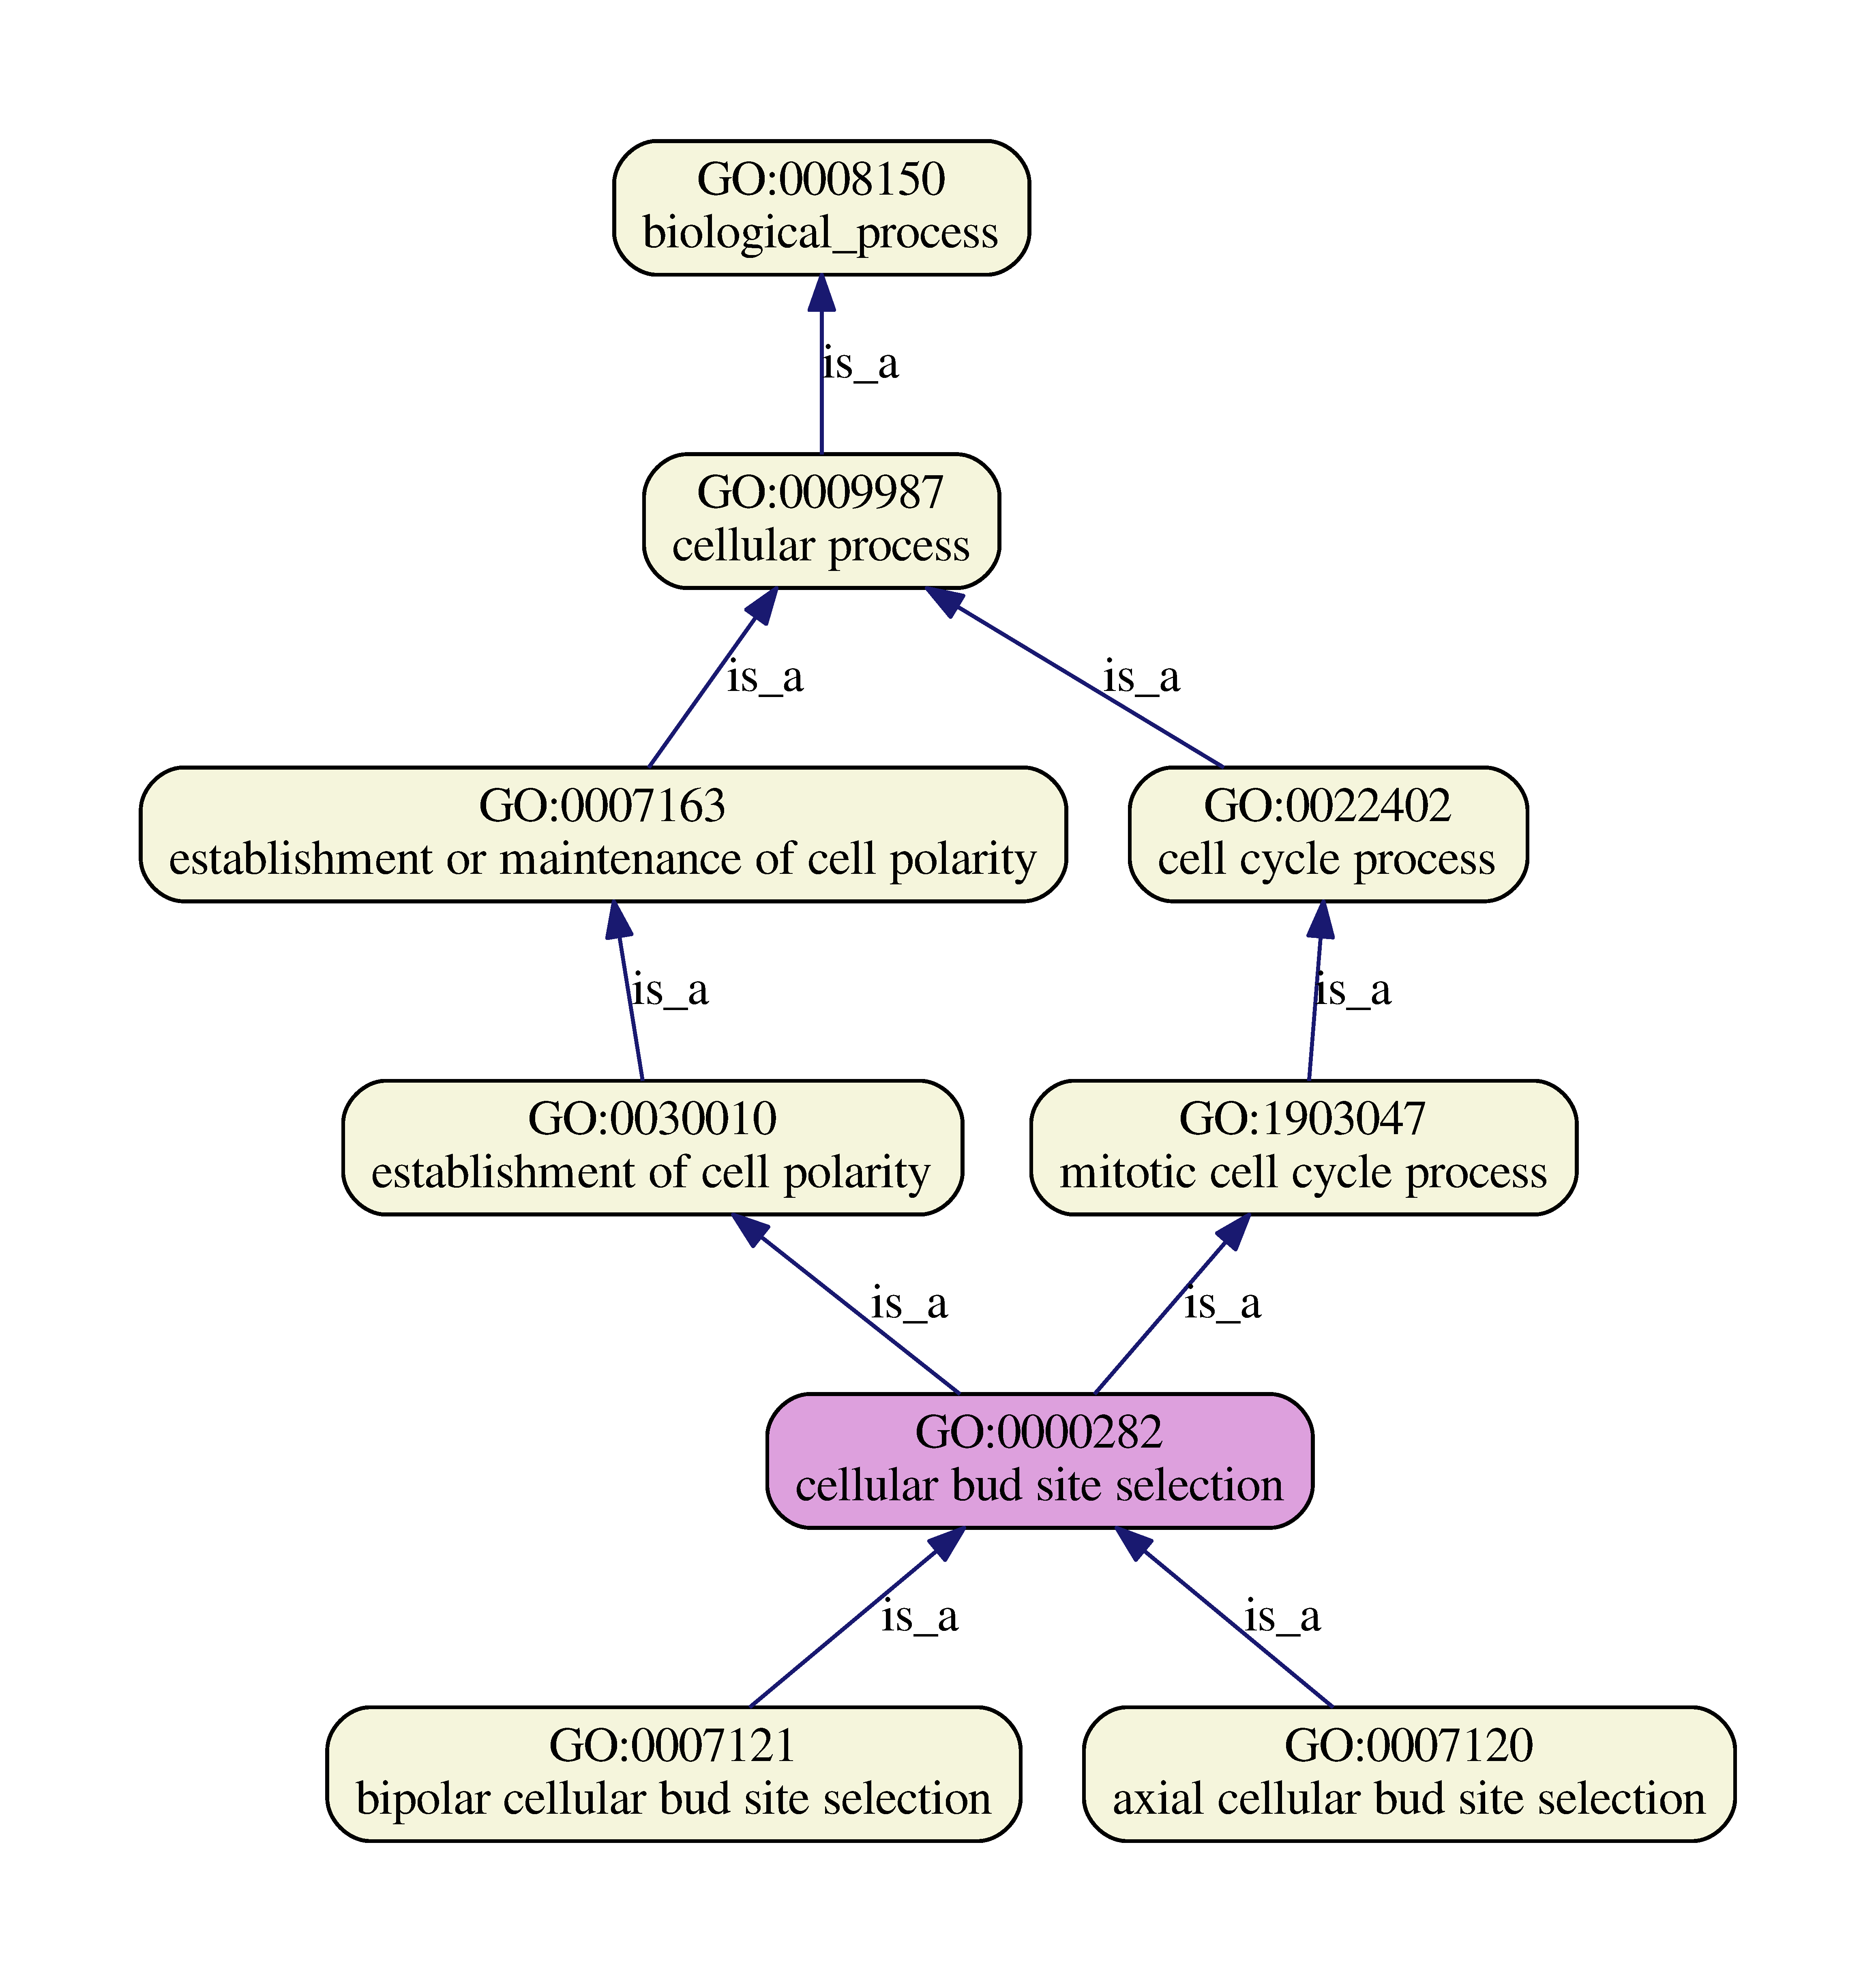
\includegraphics[width=0.49\textwidth]{ch01/demo_lineage}
  \caption[Gene ontology for \texttt{GO:0000282} or "cellular bud site selection"]{
      Gene ontology for cellular bud site selection (\texttt{GO:0000282})
      showing its relationship with respect to the parent and child classes.
  }
  \label{demo:yeast_go}
\end{figure}

\par It is evident from \texttt{GO:0000282}'s ontology that hierarchical
relationships exist between protein functions. This research strictly
focuses on multi-label classification without accounting for label
hierarchy. The benchmark datasets employed in this work and in existing literature
have independent, multiple labels. Still, classification in the presence
of multiple labels is no trivial task, and it is important to understand common 
techniques for overcoming this problem.

\subsection{Multi-label classification}

\par In typical classification tasks, two kinds of data are presented:
the \textit{features}, denoted by the matrix $\mathbf{X} =
(\mathbf{x}_{1}, \mathbf{x}_{2}, \dots, \mathbf{x}_{N})$, describing
a measurable characteristic from the system being observed, and the
\textit{labels}, denoted by the matrix $\mathbf{y} = (y_{1}, y_{2}, \dots
y_{N})$, categorizing the features into classes. A sample $i$
can be defined as a joint feature-label pair $(\mathbf{x}_{i}, y_{i})$ and a
dataset $D$ with $N$ samples can then be described as $N$ pairs of feature
and label vectors  $\{(\mathbf{x}_{i}, y_{i})\}_{i=1}^{N}$.

\par Labels are scalar values $y_{i} \in \{0, 1, 2, \dots C\}$ where each digit 
corresponds to a particular class (e.g. for image classification, $0$ is
``person'', $1$ is ``sea'', $2$ is ``boat'' and so on). The goal of
classification is to learn a hypothesis function $h$ such that it minimizes a
cost function $J$. Recall that in this task, only a single class is associated
to a particular sample. Clearly, this does not represent the case of proteins,
given that multiple classes are associated to it. Imagine a picture of a beach:
one can observe not only the ``sea'' nor the ``person,'' but both of them
existing in the same image as shown in Figure \ref{demo:multilabel}.

\begin{figure}[!t]
  \centering
  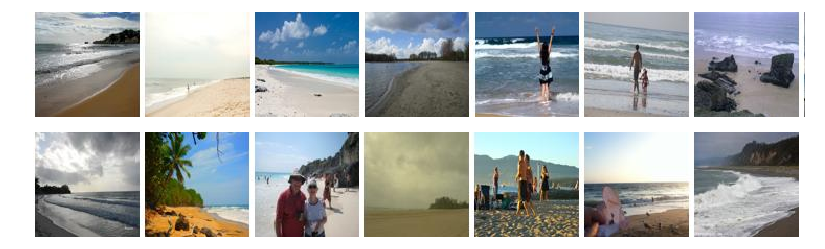
\includegraphics[width=0.70\textwidth]{ch01/demo_multilabel}
  \caption[Example of multi-label data in image scenes from MIT
  Places dataset]{
      Example of multi-label data in image scenes from the MIT
      Places dataset (\cite{zhou2014learning})}
  \label{demo:multilabel}
\end{figure}

\par For multi-label datasets, labels are often defined by vectors instead of
scalars. Here, the notation $\mathbf{Y}$ denotes the whole label matrix
containing $\mathbf{Y} = (\mathbf{y}_{1},\mathbf{y}_{2}, \dots,
\mathbf{y}_{N})$ labelsets for all samples $N$. Each sample $i$ is now defined
by a joint pair of vectors $(\mathbf{x}_{i}, \mathbf{y}_{i})$ rather than a
vector-scalar as seen in a single-label classification task. Thus for each
labelset $\mathbf{y}_{i}$ of size $L$, there exists $\mathbf{y}_{i} =
(\lambda_{1}, \lambda_{2}, \dots, \lambda_{L})_{i}$ where $\lambda_{l} \in \{0,
1\}$. The value $L$ corresponds to the number of possible labels $\lambda_{l}$
in the whole dataset. For a given protein sample, a value of $\lambda_{l}=1$
means that it performs the function $l$, whereas $\lambda_{l}=0$ means
otherwise.

\par There are two main approaches in classifying multi-label data: first by
\textit{problem transformation}, where a multi-label problem is transformed
into separate single-label classification tasks, and the second is
\textit{algorithm adaptation}, where a classifier is designed to 
directly handle multi-label data (\cite{tsoumakas2007multilabel}). This
research will focus on problem transformation, primarily because it is easier
to treat the classifier and the feature extractor as separate modules: the
classifier can be de-coupled from the feature extractor, enabling the former
to be tested on different variants of the latter.  Another reason is that the
literature on problem transformation techniques is extensive enough to
enable benchmark comparisons with different multi-label classifiers in the
future (\cite{zhang2014review, madjarov2012extensive}). The extent
of this work focuses on a specific technique called \textbf{binary relevance},
and will be treated as the baseline during the experiments.

\par Binary relevance (BR) is a problem transformation technique that
decomposes a multi-label problem into a series of single-label classification
tasks (\cite{boutell2004learning, tsoumakas2007multilabel}). This means that a
classifier $h$ is trained on each label $\lambda_l$ of $\mathbf{Y}$, training
a total of $L$ classifiers. Further modifications can be done to binary
relevance such as training a combination of labels, or building chains of
classifiers (\cite{read2009classifier}). However, due to BR's conceptual
simplicity and time-complexity\footnote[2]{
    Most problem-transformation techniques have an overhead time-complexity
    depending on the classifier $h$. For Binary relevance, we have $\bigO(L
    \cdot h(N, M))$. At inference, the complexity is $\bigO(L
    \cdot h'(M))$. This is relatively faster compared to Classifier Chains
    $\bigO(L \cdot h(N, M + L))$ or Label Ranking $\bigO(L^{2} \cdot h(N, M))$
    (\cite{zhang2014review}).
}, it has been widely used
in most literature (\cite{zhang2017binary}).

\par This research will concentrate on finding good representations for the
binary relevance classifier to solve the problem of protein function
prediction. Specifically, a binary relevance Support-Vector Machine (SVM) will
be utilized. This process of obtaining new features from raw data is called 
\textit{feature extraction} and will be one of the core ideas in this work. Even
if a BR classifier can stand on its own, it is hypothesized that higher
performance is achievable when using the extracted features as compared to the
raw data itself.

\subsection{Feature Extraction}

\par Feature extraction can be best illustrated with the \texttt{XOR} gate.
Here, we take its two inputs $\mathbf{x}_{i} = (x_{1}$, $x_{2})_{i}$ as features
and its output $y_{i} \in \{0,1\}$ as the label. With $N=4$ samples
representing all possible bit-combinations, a ``dataset''
$D=\{(\mathbf{x}_{i}, y_{i})\}_{i=1}^{4}$ can be constructed as:

\[
    D = \{(0,0,0), (0,1,1), (1,0,1), (1,1,0)\}
\]

Assuming we only have access to a linear classifier, the feature-space shown
in Figure  \ref{demo:xor} (\textit{left}) proves that classifying the samples is
difficult due to its linear inseparability\textemdash that is, drawing a single
line to perfectly separate the \texttt{X}'s and \texttt{O}'s is impossible.
However, if a new feature-space $\mathbf{\widehat{x}}$ is engineered in such a
way that $\mathbf{\widehat{x}} = (\widehat{x}_{1}, \widehat{x}_2)$ where 
$\widehat{x}_{1} = \text{\texttt{AND}}(\bar{x}_{1}, x_{2})$ and $\widehat{x}_{2}
= \text{\texttt{AND}}(x_{1}, \bar{x}_{2})$, then it is possible to transform $D$
into dataset $\widehat{D}=\{(\mathbf{\widehat{x}}_{i}, y_{i})\}_{i=1}^{4}$
where:

\[
    \widehat{D} = \{(0,0,0), (1,0,1), (0,1,1), (0,0,0)\}
\]

\noindent it can be seen from Figure \ref{demo:xor} (\textit{right}) that 
$\widehat{D}$ is a linearly separable problem solvable by any simple classifier.
In this demonstration, it is evident that hand-engineering features, or
\textit{extracting new features} has been helpful. However, with large
datasets, it will be tedious to manually find useful representations from data.
It is much preferred to automate the whole process. Note that  using this
technique is similar to finding a direct encoding from raw inputs to their 
representation. If there is no context of $\mathbf{\widehat{x}}$'s form, then
there's a need to learn a function $f$ such that $f: \mathbf{x} \rightarrow 
\mathbf{\widehat{x}}$.

\begin{figure}[!b]
  \centering
  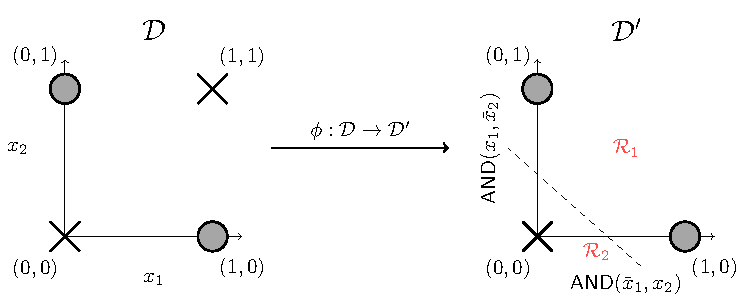
\includegraphics[width=0.70\textwidth]{ch01/demo_xor}
  \caption[Illustration of feature extraction using the \texttt{XOR} gate]{
      Illustration of feature extraction using the \texttt{XOR} gate. Using the
      raw data gives us a linearly inseparable problem \textit{(left)}.
      Constructing new features from raw data transforms the problem into a
      linearly separable one \textit{(right)}
  }
  \label{demo:xor}
\end{figure}

\subsubsection{The basic autoencoder}


\par This research proposes a feature extraction technique based on the
autoencoder neural network. As a prerequisite, it is necessary to understand
how a basic autoencoder shown in Figure \ref{schema:autoencoder} works.
Here, the function $f$ is obtained by learning a parametric map that directly
encodes the inputs to their representation (\cite{hinton1994autoencoders}).
This method relies on the features $\mathbf{X}$, unlocking correlations and 
relationships that may not be easy to find manually. The literature considers
this kind of technique as \textit{unsupervised learning} 
(\cite{bengio2013representation}).

\par Given a feature set $\mathbf{X}$, the aim is to find a set of parameters
$\theta$ such that the composite function $(g_{\theta'} \circ f_{\theta})
(\mathbf{X})$ minimizes the reconstruction error:

\[
    J(\theta) = L(\mathbf{X}, g_{\theta'}(f_{\theta}(\mathbf{X})))
\]

\noindent Here, the functions $f$ and $g$ are known as the encoder and decoder.
The former encodes the data into a representation $\mathbf{h} = f_{\theta}
(\mathbf{X})$ while the latter attempts to reconstruct $\mathbf{h}$ back into 
$\mathbf{X}$ via $\mathbf{\widetilde{X}} = \mathbf{X} \approx g_{\theta'}
(\mathbf{h})$. Most works implement a tied-weighing scheme (i.e,
$\theta=\theta^{T}$ between the encoder and decoder weights
(\cite{bengio2013representation}). Take note that the
size of $\mathbf{h}$ may not necessarily be the same as $\mathbf{X}$. In sum,
the autoencoder takes an input matrix and faithfully reconstructs it given a
bottleneck (the size of $\mathbf{h}$). This may sound trivial, but due to the
\textit{encoding layer}  $\mathbf{h}$, interesting structure is learned from
the data. The learned representations $\mathbf{h}$ are treated as the new
input $\mathbf{\widehat{X}}$  (similar to the \texttt{XOR} problem) for a
classifier. With a good set-up and optimization scheme, it is even possible to
compress data using this technique (\cite{theis2017lossy}).

\begin{figure}[!t]
  \centering
  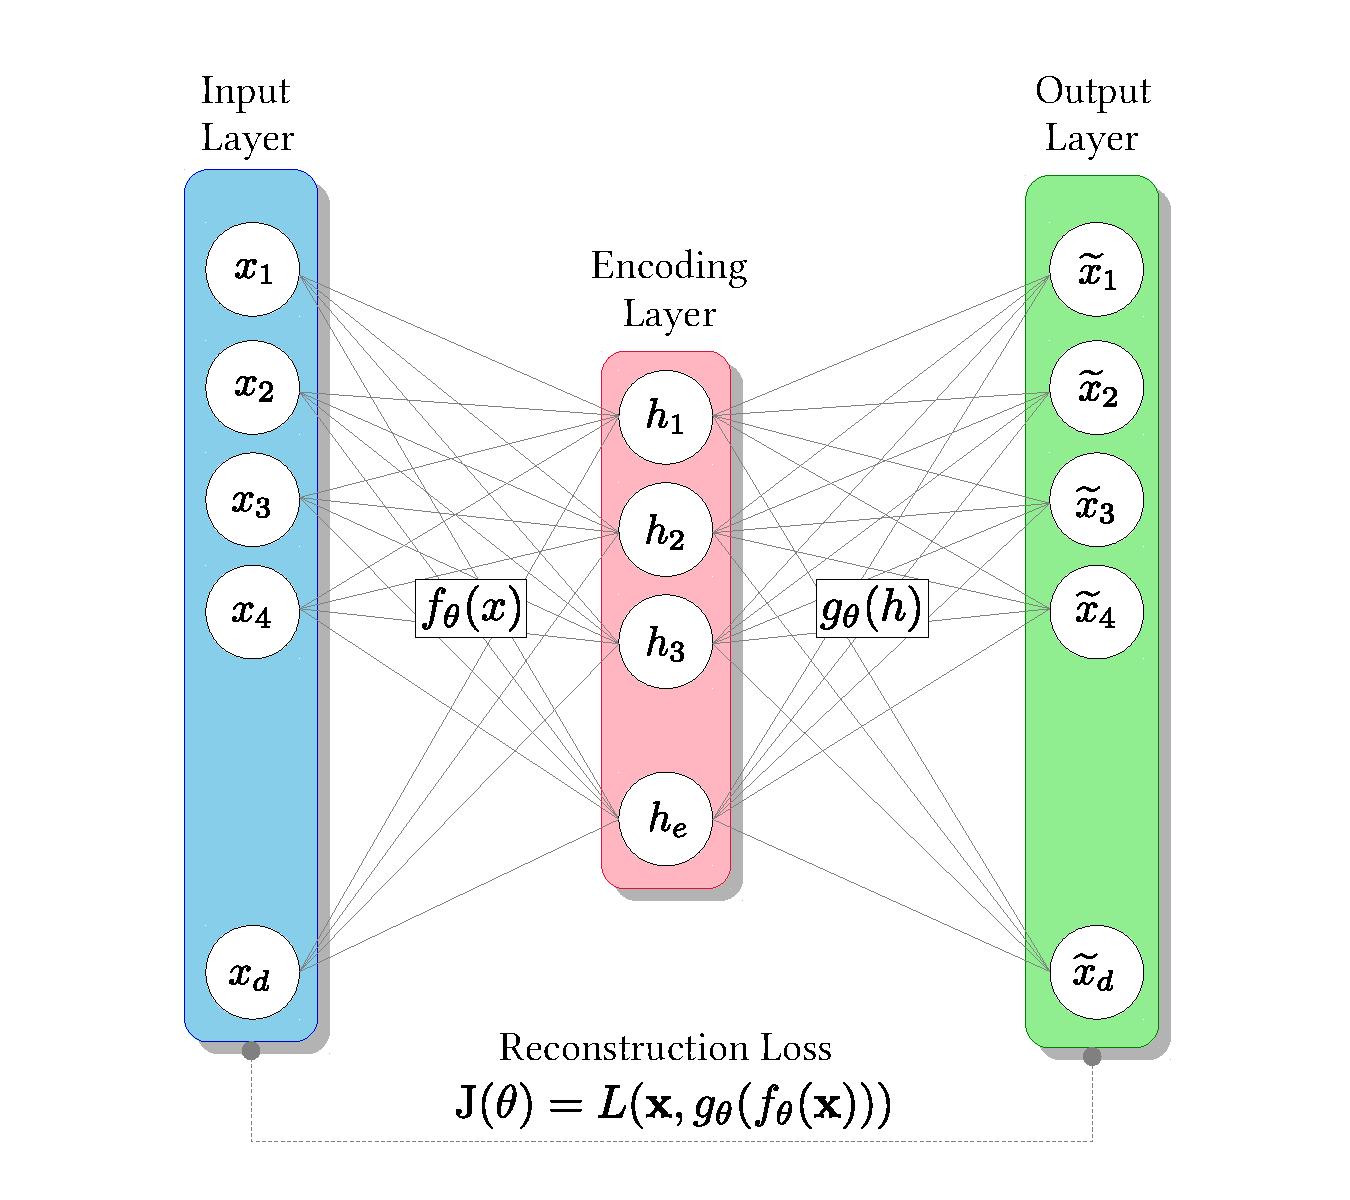
\includegraphics[width=0.60\textwidth]{ch01/schema_autoencoder}
  \caption[Diagram of the basic autoencoder]{
      Diagram of the basic autoencoder
  }
  \label{schema:autoencoder}
\end{figure}

\section{Motivation}
\label{Motivation}

\par Although extracting features using an autoencoder has been helpful for
classification, one shortcoming of this technique is its tendency to learn
trivial representations from sparse and high-dimensional data
(\cite{wang2017feature, chen2017kate})\textemdash types of data characteristic
of proteins. This is usually the case when the optimization task is to learn
an approximation to the identity $\mathbf{X} \approx \mathbf{\widehat{X}}$,
favoring irrelevant features by overfitting instead of learning a generalized
pattern or representation. Motivating the autoencoder to create relevant features
for the classification task is then important.

\par To address this issue, this work proposes an autoencoder architecture that
extracts a set of sparse yet relevant features. This is done through mutual
competition: the neurons on the network compete based on their activation, and
the ``winners'' absorb the ``losers,'' boosting their importance in the network.
Competition adjusts the backpropagation path, favoring the winners to represent
the input data. This method is task-specific for protein data because only a subset
of its features is considered useful (\cite{iqbal2014efficient, gaudet2017gene}).
The proposed method will be trained on two protein benchmark datasets, and the
extracted features will be used as input to a binary relevance classifier. It will
be compared against a baseline method without feature extraction, and opposed to
existing techniques in literature.

\section{Problem Formulation}
\label{Problem}

\par This research proposes a technique for extracting relevant features from
protein data. It also investigates the effect of feature-relevance to the
performance of a multi-label classifier. Selective feature extraction is
accomplished by encouraging competition between the neurons of an
autoencoder network. In line with this, the following questions will be
answered throughout this work:

\begin{itemize}
    \item How relevant are the learned representations from the proposed method
        as compared to the raw features? (Sec. \ref{FeatureRelevance})
    \item How well does a multi-label classifier perform when using the
        features extracted by the proposed method? (Sec. \ref{ModelQuality})
    \item How well do the hyperparameters improve the basic autoencoder and
        affect model performance? (Sec. \ref{AblationTest})
    \item How well does the proposed method compare with other techniques in
        literature? (Sec. \ref{Benchmarking})
\end{itemize}



\chapter{Literature Review}
\label{LiteratureReview}


%=============================================================================
% Methodology
% Copyright (c) 2018. Lester James V. Miranda
%
% This file is part of thesis-manuscript.
%
% thesis-mansucript is free software: you can redistribute it and/or modify
% it under the terms of the GNU General Public License as published by
% the Free Software Foundation, either version 3 of the License, or
% (at your option) any later version.
%
% thesis-manuscript is distributed in the hope that it will be useful,
% but WITHOUT ANY WARRANTY; without even the implied warranty of
% MERCHANTABILITY or FITNESS FOR A PARTICULAR PURPOSE.  See the
% GNU General Public License for more details.
%
% You should have received a copy of the GNU General Public License
% along with thesis-manuscript.  If not, see <http://www.gnu.org/licenses/>.
%
% Created by: Lester James V. Miranda <ljvmiranda@gmail.com>
%=============================================================================

\chapter{Proposed Method}
\label{Methodology}

% Write overview here, talk about the training and test phases.

\par The entire protein function prediction model consists of two stages: (1) a
\textit{feature extraction} stage that extracts new representations from
raw data, and a \textit{multi-label classification} stage that assigns each
protein sample to its respective set of functions. During training, the
model learns the parameters $\theta$ and $W$ for the two stages separately.
At inference, matrix operations are only applied to transform the input data
and predict protein functions. An illustration for the training and test phases
can be found at Figure \ref{schema:training_testing}. \footnote[2]{The subscripts
$tr$ and $ts$ refer to the training and test data respectively.} The proposed
autoencoder network resides in the first stage.

\par This chapter will discuss in detail the algorithm in Section
\ref{FeatureExtraction}, and the multi-label classifier in Section
\ref{MultiLabelClassification}. Lastly, an overview of the
datasets and experimental environment will be described in Sections
\ref{Datasets} and \ref{ExperimentalEnvironment} respectively.


\begin{figure}[h]
    \centering
    \begin{subfigure}[b]{0.8\textwidth}
        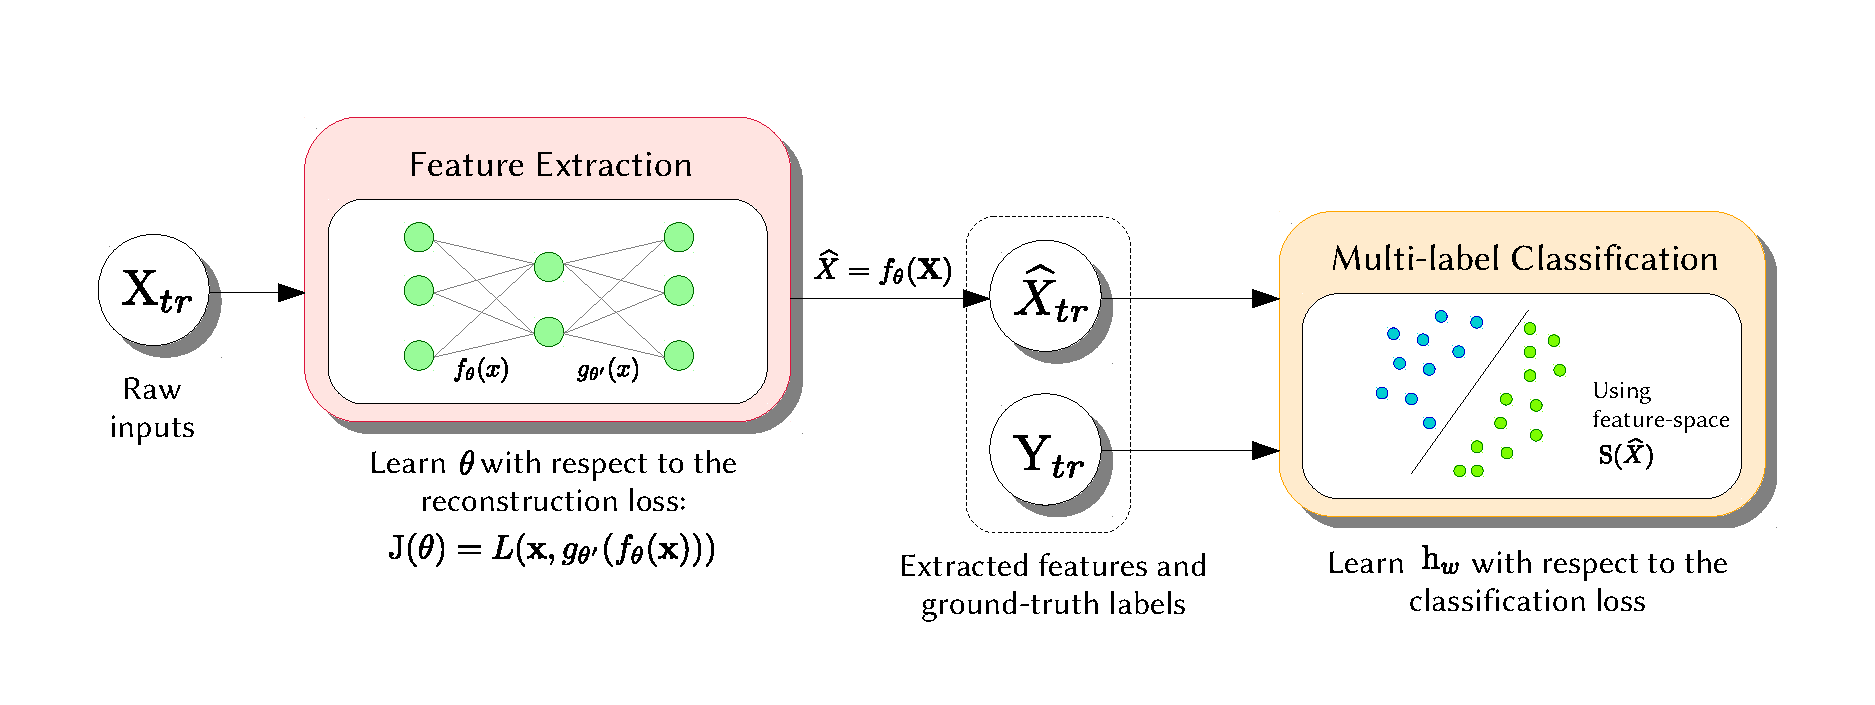
\includegraphics[width=\textwidth]{ch03/schema_training}
        \caption{Training phase}
        \label{schema:training}
    \end{subfigure}
    ~ %add desired spacing between images, e. g. ~, \quad, \qquad, \hfill etc. 
      %(or a blank line to force the subfigure onto a new line)
    \begin{subfigure}[b]{0.9\textwidth}
        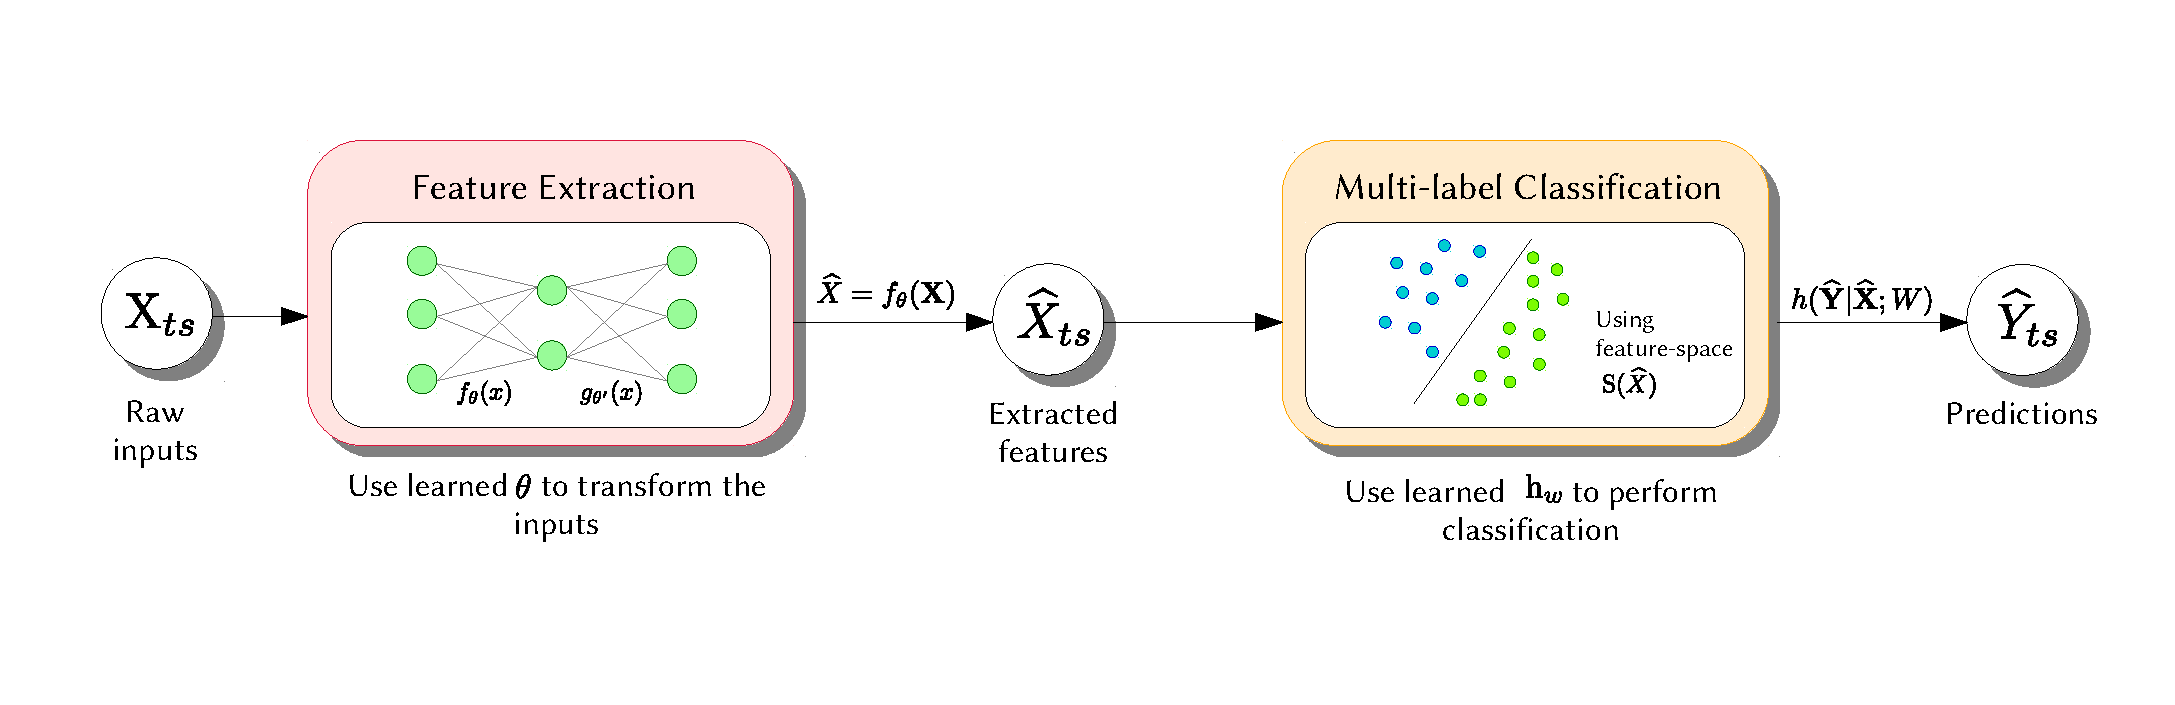
\includegraphics[width=\textwidth]{ch03/schema_testing}
        \caption{Testing phase}
        \label{schema:testing}
    \end{subfigure}
    \caption{Train and test phases for the protein function prediction model}
    \label{schema:training_testing}
\end{figure}

\section{Feature Extraction}
\label{FeatureExtraction}

\par This stage consists of the proposed autoencoder network for selective
feature extraction. Selecting relevant features is achieved through mutual
competition. All of this happens at the training phase and is accomplished
by performing the following tasks:

\begin{itemize}
    \item A winner-take-all operation selects the top k\% neurons or 
        \textit{winners} depending on their activation value; and
    \item A sparse operation redistributes the activation of the non-k\%
        neurons or \textit{losers} to the winners. This results to a sparse
        layer highlighting the winning or relevant neurons.
\end{itemize}

\noindent  Figure \ref{schema:proposed} illustrates the proposed network.
At testing, the two operations are simply turned-off. The network uses the
learned weights from training to determine and transform the relevant features
from the input test data.

\par From this design, three hyperparameters can be adjusted:

\begin{itemize}
    \item The encoding layer size, $e$, that controls how many features
        should be extracted from the raw data. (If $e>d$ then the network is
        overcomplete, otherwise it is undercomplete).
    \item The percent sparsity $k\%$ that determines the number of winners $w$
        retained during the winner-take-all operation.
    \item The competition parameter $\alpha$ that adjusts the amount of activation
        from the losers to be distributed to the winners.
\end{itemize}

\begin{figure}[h]
    \centering
    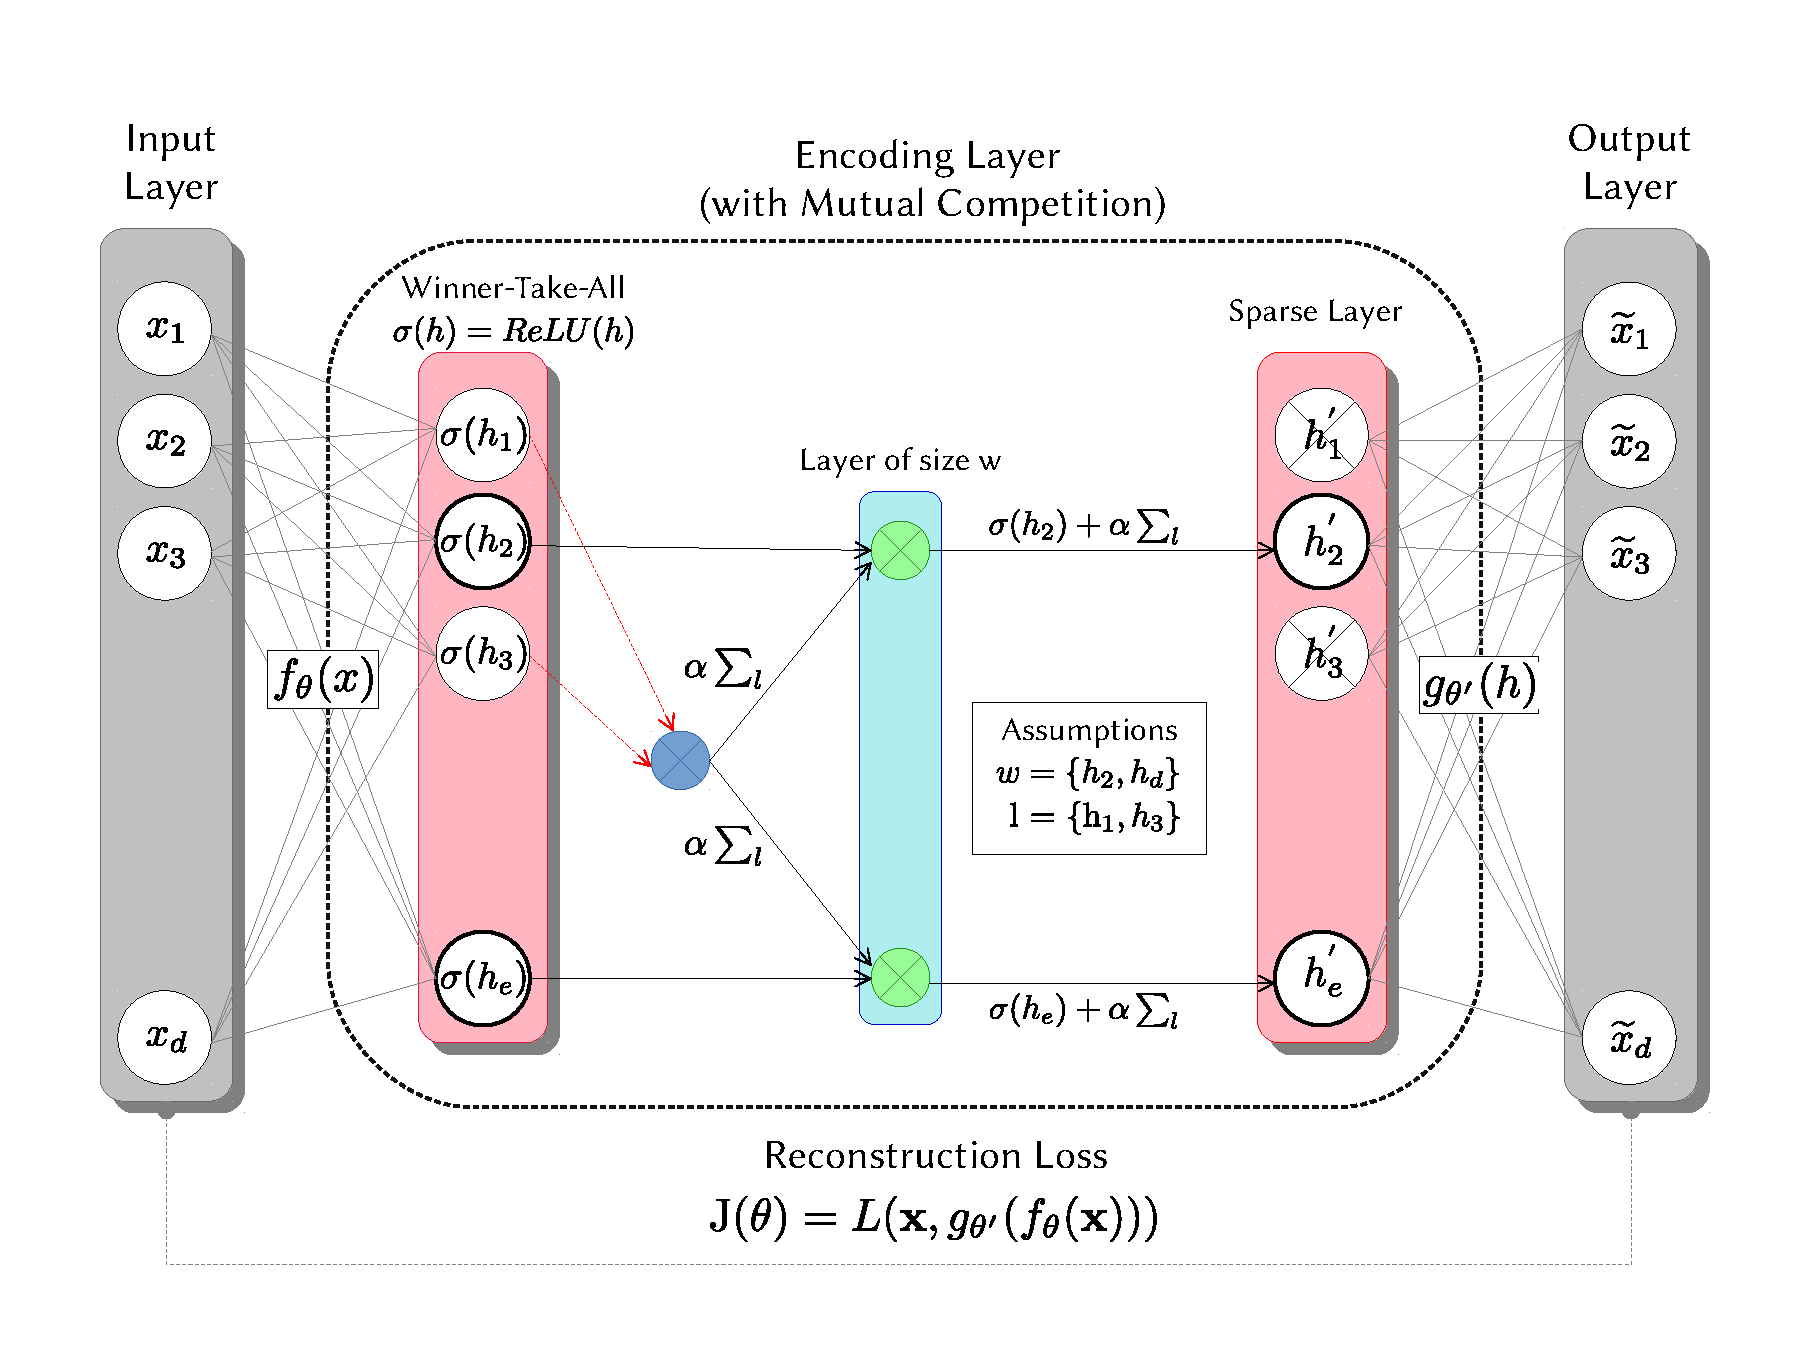
\includegraphics[width=0.75\textwidth]{ch03/schema_proposed}
    \caption[Proposed autoencoder network with mutual competition]
    {The proposed autoencoder network with mutual competition}
    \label{schema:proposed}
\end{figure}

\par Algorithm \ref{algo:training} gives an overview of the training procedure
for the proposed method. The autoencoder starts off by initializing the weight
parameters randomly from a normal distribution. Then, for a set number of
epochs, a feedforward step with ReLU activation maps the inputs $\mathbf{x}$
to the encoding dimension $\mathbf{h}$ of size $e$. A winner-take-all
operation creates a dictionary of all $k$ winners and losers to set-up the
sparse layer. The layer contains the winners with their updated
activations from the losers as controlled by $\alpha$. Afterwards, the
decoder function will attempt to reconstruct the input from the sparse layer.
This finally initiates the backpropagation routine to update the parameters
$\theta$. At the end of training, the model parameters are returned.

%=============================================================================
% algo-training.tex
% Copyright (c) 2018. Lester James V. Miranda
%
% This file is part of thesis-manuscript.
%
% thesis-mansucript is free software: you can redistribute it and/or modify
% it under the terms of the GNU General Public License as published by
% the Free Software Foundation, either version 3 of the License, or
% (at your option) any later version.
%
% thesis-manuscript is distributed in the hope that it will be useful,
% but WITHOUT ANY WARRANTY; without even the implied warranty of
% MERCHANTABILITY or FITNESS FOR A PARTICULAR PURPOSE.  See the
% GNU General Public License for more details.
%
% You should have received a copy of the GNU General Public License
% along with thesis-manuscript.  If not, see <http://www.gnu.org/licenses/>.
%
% Created by: Lester James V. Miranda <ljvmiranda@gmail.com>
%=============================================================================

\begin{algorithm}
\caption{Training the proposed autoencoder network}
\label{algo:training}
\begin{algorithmic}[1]

\INPUT Training examples $\mathbf{X}$, competition parameter $\alpha$, percent sparsity $k\%$
\OUTPUT Model weights $\theta$, extracted features $\mathbf{\widehat{X}}$

\item[]
\Procedure{Initialization}{}
    \State $\theta_{i}^{(0)} \gets \mathcal{N}(\mu,\,\sigma^{2})$
    \Comment{Initialize weights}
    \State $\theta_{0}^{(0)} \gets \mathcal{N}(\mu,\,\sigma^{2})$
    \Comment{Initialize biases}
\EndProcedure

\item[]
\Procedure{Training}{}
    \For{\textit{NumEpochs}}
        \State Feedforward propagation: $\mathbf{h} \gets f_{\theta}(\mathbf{X}) =
        \sigma(\theta\mathbf{X}^{T}+\theta_{0})$
        \Comment Until last encoding layer
        \State $D \gets$ \Call{WinnerTakeAll}{$\mathbf{h}$, $k$}
        \Comment Store winners and losers in a dictionary
        \State $\mathbf{h'} \gets$ \Call{Sparse}{$D$, $\alpha$}
        \State Compute output: $\mathbf{\widetilde{X}} \gets 
        g_{\theta'}(\mathbf{h'}) = \sigma(\theta'\mathbf{h'}^{T}+\theta_{0})$
        \Comment Tied weights, $\theta'=\theta^{T}$
        \State Compute reconstruction error $\mathbf{J}_{\theta}$
        \State \Call{Backpropagation}{$\mathbf{J}_{\theta}$}
        \Comment Only for winning neurons
    \EndFor
    \State \Return $\theta$ 
\EndProcedure

\item[]
\Procedure{Transform}{$\mathbf{X}$}
    \State
    $\mathbf{\widehat{X}}=f_{\theta}(\mathbf{X})=\sigma(\theta\mathbf{X}^{T} +
    \theta_{0})$
    \State \Return $\mathbf{\widehat{X}}$
\EndProcedure

\end{algorithmic}
\end{algorithm}


\par When performing a feature transform, we use the encoder function
$f_{\theta}$ to map the input into its new representation. The extracted
features $\mathbf{\widehat{X}}$ has a size $e$ as determined from training.
The winner-take-all and sparse operations are turned-off during this process.
Further details on these operations will be discussed in the proceeding
sections.

\subsection{Winner-take-all operation}

\par The winner-take-all operation retains the top $k$\% neurons
in a given layer based on its activation. Thus, after the feedforward phase,
instead of directly reconstructing the encoded data, a percentage of
neurons in the last encoding layer are kept by the network. In this manner, a
lifetime sparsity is enforced and the rest of the non-$k$\% neurons
(or ``losers'') are set to $0$ by the sparse operation later.

\par During the backpropagation phase, the error is only passed through
the non-zero neurons in the hidden layers. When performing a feature transform
, this operation is ignored. Since the weights were trained with
respect to the ``winners,'' it enables the model to distinguish the
corresponding neurons. Algorithm \ref{algo:wta} describes this procedure.

%=============================================================================
% algo_wta.tex
% Copyright (c) 2018. Lester James V. Miranda
%
% This file is part of thesis-manuscript.
%
% thesis-mansucript is free software: you can redistribute it and/or modify
% it under the terms of the GNU General Public License as published by
% the Free Software Foundation, either version 3 of the License, or
% (at your option) any later version.
%
% thesis-manuscript is distributed in the hope that it will be useful,
% but WITHOUT ANY WARRANTY; without even the implied warranty of
% MERCHANTABILITY or FITNESS FOR A PARTICULAR PURPOSE.  See the
% GNU General Public License for more details.
%
% You should have received a copy of the GNU General Public License
% along with thesis-manuscript.  If not, see <http://www.gnu.org/licenses/>.
%
% Created by: Lester James V. Miranda <ljvmiranda@gmail.com>
%=============================================================================


\begin{algorithm}
    \caption{Winner-Take-All operation}
    \label{algo:wta}
    \begin{algorithmic}[1]
    
    \INPUT Output of last encoding layer $\mathbf{h}$, percent sparsity $k\%$
    \OUTPUT Dictionary of winners and losers, $D = \{\}$

    \item[]
    \State \textit{LayerSize} $\gets$ length($\mathbf{h}$)
    \Comment Get number of units in the layer
    \State \textit{NeuronsToKeep} $\gets k\% * \text{\textit{LayerSize}}$
    \State $D[\text{Winners}] \gets$ first \textit{NeuronsToKeep} in \Call{SortAscendingOrder}{$\mathbf{h}$}
    \State $D[\text{Losers}] \gets$ remaining neurons in \Call{SortAscendingOrder}{$\mathbf{h}$}
    \State \Return $D$
    \end{algorithmic}
\end{algorithm}


\subsection{Sparse operation}

\par The sparse operation allows the winner neurons to ``soak-up'' the
activation of the loser neurons. This is done via an adder controlled by
a hyperparameter $\alpha$. Boosting the energy of the winning neurons can
affect the backpropagation path so that weights are optimized in their favor.
This assumes that the winners, due to their high activation, are the
relevant features representing the input data. Algorithm \ref{algo:sparse}
describes this operation.

%=============================================================================
% algo_sparse.tex
% Copyright (c) 2018. Lester James V. Miranda
%
% This file is part of thesis-manuscript.
%
% thesis-mansucript is free software: you can redistribute it and/or modify
% it under the terms of the GNU General Public License as published by
% the Free Software Foundation, either version 3 of the License, or
% (at your option) any later version.
%
% thesis-manuscript is distributed in the hope that it will be useful,
% but WITHOUT ANY WARRANTY; without even the implied warranty of
% MERCHANTABILITY or FITNESS FOR A PARTICULAR PURPOSE.  See the
% GNU General Public License for more details.
%
% You should have received a copy of the GNU General Public License
% along with thesis-manuscript.  If not, see <http://www.gnu.org/licenses/>.
%
% Created by: Lester James V. Miranda <ljvmiranda@gmail.com>
%=============================================================================

\begin{algorithm}
    \caption{Sparse operation}
    \label{algo:sparse}
    \begin{algorithmic}[1]
    
    \INPUT Dictionary of winners and losers $D = \{\}$, competition parameter $\alpha$
    \OUTPUT Updated activation of winners and losers $\mathbf{h}'$

    \item[]
    \State \textit{ToAllocate} $\gets$ \Call{Sum}{$D[Losers]$}
    \Comment Sum all activations of loser neurons
    \State $\mathbf{a}_{w} \gets$ $D[Winners]$ + $\alpha$ \textit{ToAllocate}
    \Comment Update activation of winners, $\mathbf{a}_{w}$
    \State $\mathbf{a}_{l} \gets 0$ 
    \Comment Set activation of losers to $0$.
    \State \textbf{return} $\mathbf{h}' = \{\mathbf{a}_{w}$, $\mathbf{a}_{l}\}$
    \end{algorithmic}
\end{algorithm}


\section{Multi-label Classification}
\label{MultiLabelClassification}

\par Once extracted, the new features will be sent to a multi-label classifier for
inference. We train the classifier $h$, and learn its parameters $W$. In this
research, $h$ comes in the form of a binary-relevance support-vector machine
(BR-SVM), and is trained with respect to the SVM squared hinge loss (L2-SVM): 

\begin{equation}
J_i = \sum_{\widehat{\mathbf{y}}_i \neq \mathbf{y}_i}\max(0, W_{\widehat{\mathbf{y}}}^{T} \mathbf{x}_{i}^{'} - W_{\mathbf{y}_i}^{T}\mathbf{x}_{i}^{'} + \Delta)^{2}
\end{equation}

\par During SVM training, two library implementations were used: LIBSVM and
LIBLINEAR for the gaussian and linear kernels respectively
(\cite{chang2011libsvm, fan2008liblinear}). However, given large datasets, the
SVM algorithm can reach a time-complexity between $\mathcal{O}(n^{2})$ and
$\mathcal{O}(n^{3})$ (\cite{bottou2006support}). If we account for the
additional complexity of binary-relevance for each label, then the overall
training time will be longer. To resolve this problem, distributed training was
implemented.

\par Figure \ref{schema:multiprocessing} outlines this procedure. The training
dataset was partitioned into $N$ batches, and was distributed to $N$ jobs. The
protein samples for each partition were chosen randomly without replacement and
is assigned into its own thread. Because there are less number of samples for
each SVM classifier, training becomes much faster. Finally, the validation score
is obtained by averaging the results of all partitions for each label
$\lambda$. This results to a trained classifier $h(\mathbf{Y} \given
\mathbf{\widehat{X}}; \mathbf{W})$ for inferring the test data.

\begin{figure}[t]
    \centering
    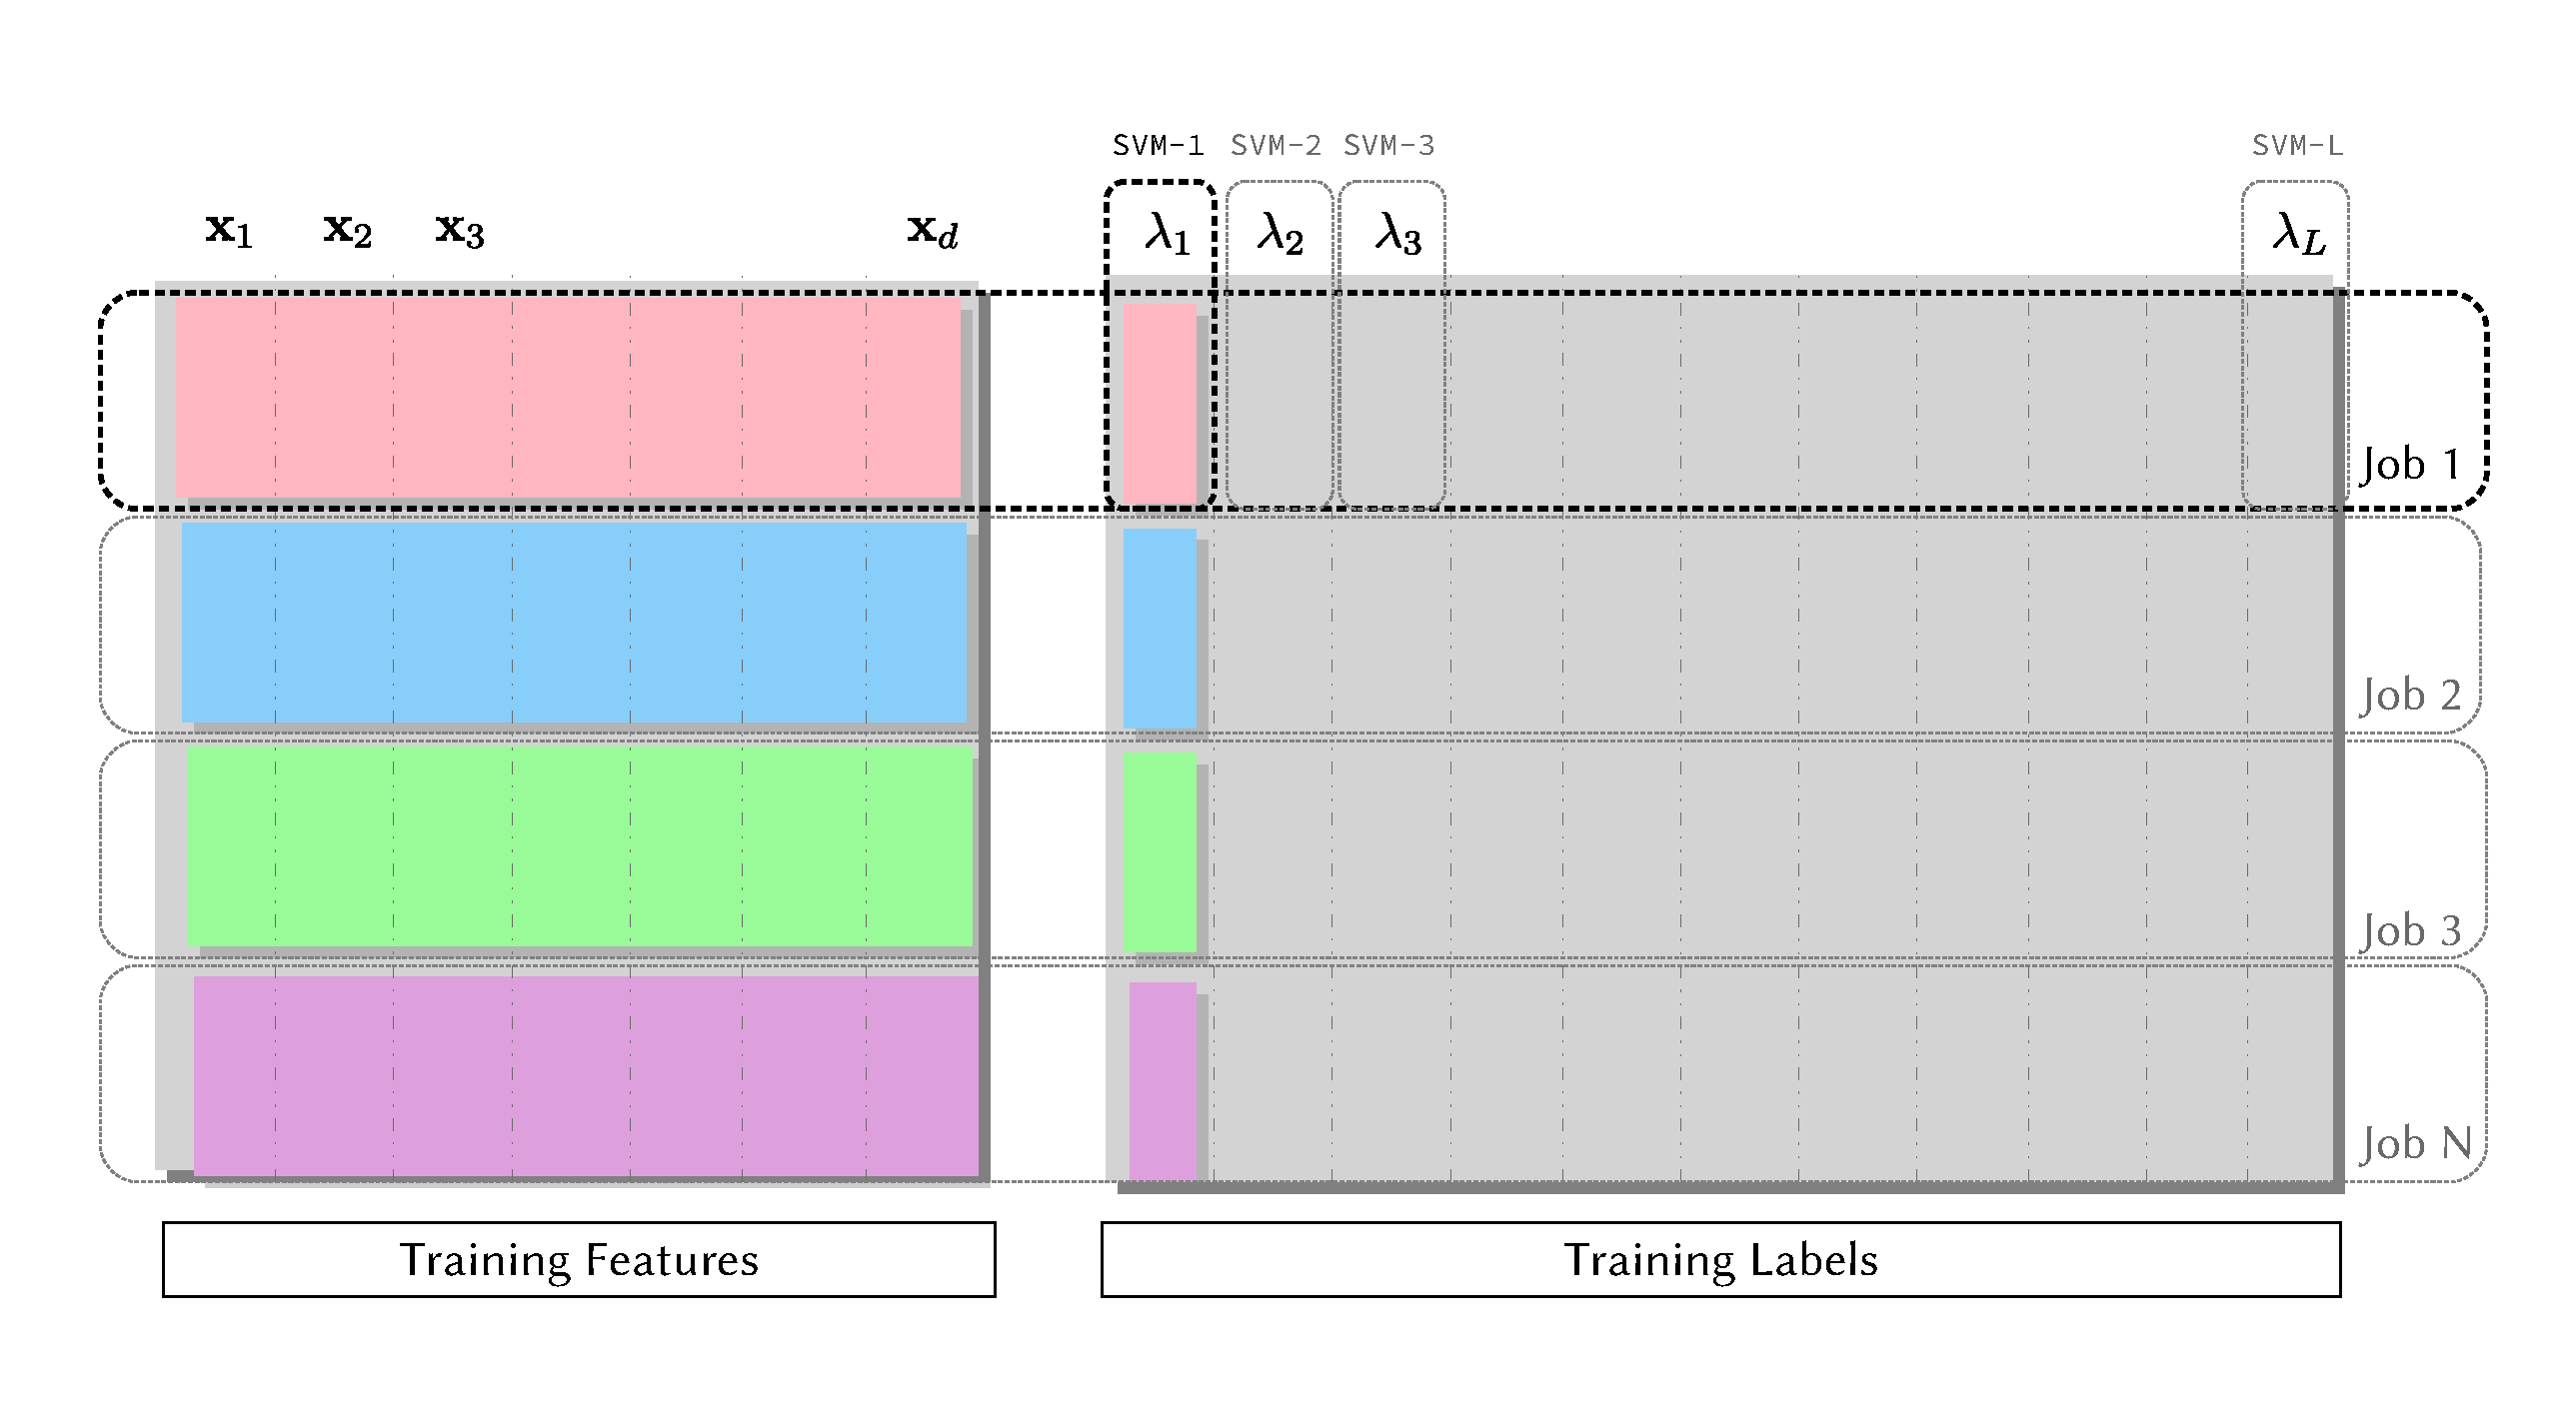
\includegraphics[width=0.75\textwidth]{ch03/schema_multiprocessing}
    \caption[Distributed approach in training multiple BR-SVMs]
    {Distributed approach in training multiple BR-SVMs. The training dataset
    was partitioned into $N$ jobs where each is assigned into a thread.}
    \label{schema:multiprocessing}
\end{figure}

\subsection{Evaluation Metrics}

To evaluate the performance of the prediction model, we will use the following
metrics\footnote[2]{\textit{tp}: true positive, \textit{fp}:
false positive, \textit{tn}: true negative, \textit{fn}: false negative}:

\begin{align}
    \text{Hamming Loss (H)} &= \dfrac{1}{N \cdot L} \sum_{i=1}^{N} \sum_{j=1}^{L}
    \text{XOR}(y_{ij}, \widehat{y}_{ij}) \\
    \text{Precision (P)} &=
    \dfrac{1}{N}\sum_{i=1}^{N}\dfrac{|\mathbf{\widehat{y}}_{i} \cap
    \mathbf{y}_{i}|}{|\mathbf{\widehat{y}_{i}}|} = \dfrac{tp}{tp + fp} \\
    \text{Recall (R)} &=
    \dfrac{1}{N}\sum_{i=1}^{N}\dfrac{|\mathbf{\widehat{y}}_{i} \cup
    \mathbf{y}_{i}|}{|\mathbf{\widehat{y}_{i}}|} = \dfrac{tp}{tp + fn} \\
    \text{F-score (F)} &=
    \dfrac{1}{N}\sum_{i=1}^{N} \dfrac{2 | \mathbf{\widehat{y}}_{i} \cup
        \mathbf{y}_{i}|}{|\mathbf{\widehat{y}}_{i} | + |\mathbf{y}_{i}|} =
        \dfrac{2 (\text{P} \cdot \text{R})}{\text{P} +
        \text{R}}
\end{align}

\par We will also compute for a fifth metric, the Area Under the ROC Curve
(AUROC), to serve as proxy for accuracy. Together with the Hamming loss and
F-score, the model will be evaluated and compared to other works. Lastly,
the Precision-Recall score will determine the quality of our model in terms of
sensitivity and specificity.

\par In addition, the AUROC, F-score, and Precision-Recall will be averaged
in three ways: micro (\textit{mi}), macro (\textit{ma}), and by-samples
(\textit{sa}). As an illustration, given $L$ labels and $N$ samples, a
micro-averaged precision ($P_{mi}$) is computed using the true-positives and
false-positives of each label and averaged:

\[
    P_{mi} = \dfrac{\sum_{i=1}^{L} tp_{i}}{\sum_{i=1}^{L} tp_{i} +
    \sum_{i=1}^{L} fp_{i}}
\]

\noindent In macro-averaging, the precision for each label is computed and
averaged. Because this metric is weighted, they are affected by
the number of true instances for each label $l$. This weighing scheme
offsets class imbalance:

\[
    P_{ma} = \dfrac{1}{L} \sum_{i=1}^{L} w_{i} P_{i}
\]

\noindent Lastly, in samples averaging, the metrics are computed for each
instance $m$ and averaged by the number of samples:

\[
    P_{samples} = \dfrac{1}{M}\sum_{i=1}^{M} P_{i}
\]

\noindent Averaging in this manner creates a stricter set of metrics
consistent with other works in literature (\cite{madjarov2012extensive,
gibaja2015tutorial, herrera2016multilabel, tsoumakas2017data}).

\section{Datasets}
\label{Datasets}

\par Two benchmark datasets will be studied in this work. First is the
\textbf{yeast} dataset that contains micro-array expression data and
phylogenetic profiles of 1500 genes in \textit{Saccharomyoes cerevisiae} or
baker's yeast (\cite{elisseeff2001kernel}). Second is the \textbf{genbase}
dataset containing protein sites and motif data of the ten most important
protein families\footnote[2]{The protein families are described in terms of
their Prosite documenation ID (\cite{diplaris2005protein,
bairoch1991prosite,hatzidamianos2003genminer}): PDOC00064 (oxydoreductases),
PDOC00154 (isomerases), PDOC00224 (cytokines and growth factors), PDOC00343
(structural proteins), PDOC00561 (receptors), PDOC00662 (DNA or RNA associated
proteins), PDOC00670 (transferases), PDOC00791 (protein secretion and
chaperones), and PDOC50007 (hydrolases).} (\cite{diplaris2005protein}). Table
\ref{setup:datasets} provides their description.

\par Recall that labelsets are represented as a binary matrix $\mathbf{Y} \in
\{0,1\}^{M \times N} $ where $\lambda_{mn} = 1$ if protein sample $m$ has
function $n$ and $0$ otherwise. Here, cardinality represents the average
number of active labels ($\lambda_{mn}=1$) per instance. Thus, a $4.237$ value
in yeast indicates that each sample is associated with slightly more than $4$
labels on average. On the other hand, density describes labelset sparsity. A
value of $0.0460$ in genbase means that around $4.6\%$ of labels are active.

\par To illustrate the multi-label aspect of the two datasets, Figure
\ref{graph:cooccurence} shows a co-occurence plot. Each arc in the circle
corresponds to a protein function in the dataset. The width of the arc
represents its frequency. Each chord connecting any two arcs depicts their
simultaneous presence in a protein sample.


\begin{table}[t]
    \centering
    \caption{Dataset description}
    \label{setup:datasets}
    \begin{tabular}{@{}rrrrrr@{}}
        \toprule
        Dataset & Instances & Features & Labels & Cardinality & Density    \\ \midrule
        yeast   & $2417$      & $103$      & $14$     & $4.237$       & $0.3030$     \\
        genbase & $662$       & $1186$     & $27$     & $1.252$       & $0.0460$     \\ \bottomrule
    \end{tabular}
\end{table}


\begin{figure}[t]
    \centering
    \begin{subfigure}[b]{0.49\textwidth}
        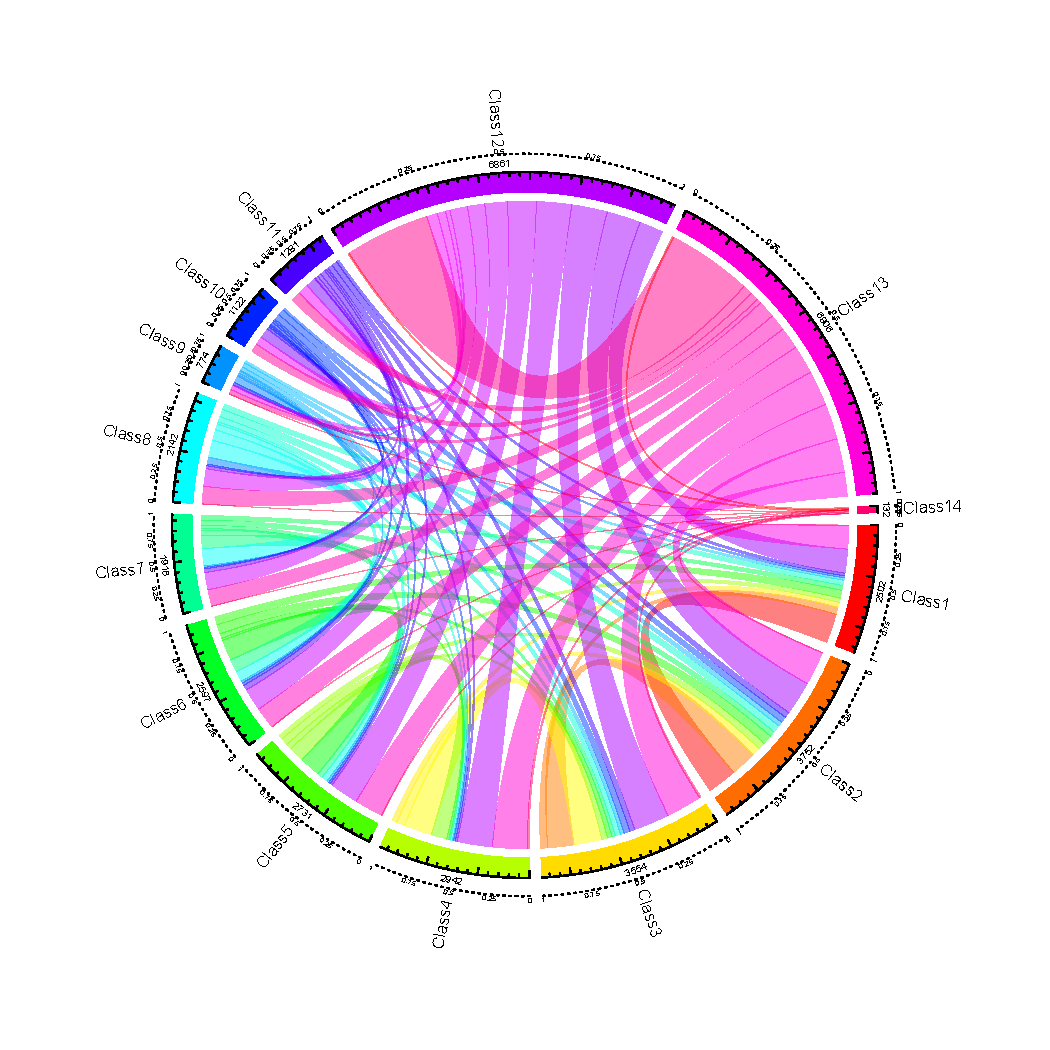
\includegraphics[width=\textwidth]{ch03/graph_yeast}
        \caption{Yeast}
        \label{graph:yeast}
    \end{subfigure}
    ~ %add desired spacing between images, e. g. ~, \quad, \qquad, \hfill etc. 
      %(or a blank line to force the subfigure onto a new line)
    \begin{subfigure}[b]{0.49\textwidth}
        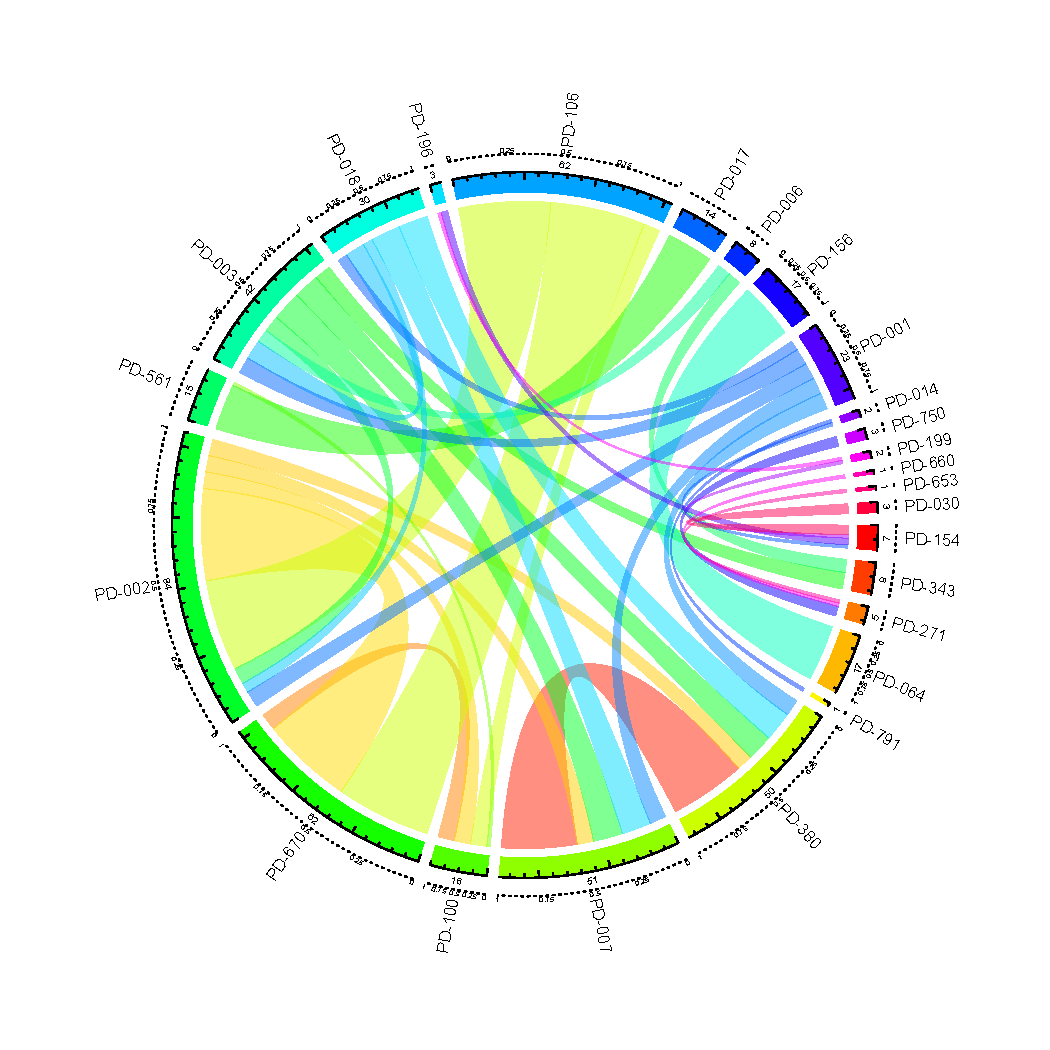
\includegraphics[width=\textwidth]{ch03/graph_genbase}
        \caption{Genbase}
        \label{graph:genbase}
    \end{subfigure}
    \caption{Co-occurence plot for the yeast and genbase datasets.}
    \label{graph:cooccurence}
\end{figure}

\section{Experimental Environment}
\label{ExperimentalEnvironment}

Table \ref{setup:environment} describes the environment used for the
experiments. The source code can be obtained from
\url{https://github.com/ljvmiranda921/PFPredict}.

\begin{table}[h]
    \centering
    \caption{Experimental Environment}
    \label{setup:environment}
    \begin{tabular}{@{}rl@{}}
        \toprule
        Environment             & Value                  \\ \midrule
        \textit{Validation and testing}                  \\ 
        Nb. of trials           & $10$                   \\
        Train-test split        & $80-20$                \\
        Validation              & k-fold ($k=5$)         \\
        \textit{Hardware dependencies}                   \\
        Nb. of cores            & 40                     \\
        GPU                     & NVIDIA Titan X         \\ 
        CPU                     & Intel Xeon 2.2GHz      \\
        \textit{Software dependencies}                   \\
        Language                & Python 2.7, 3.6        \\
        Libraries               & Tensorflow 1.2.1, Keras 2.1.2 \\ \bottomrule
    \end{tabular}
\end{table}





\chapter{Results and Discussion}
\label{Results}

Four (4) sets of experiments were performed to test the proposed method.
Each answers a question as posed in Section \ref{Problem}.
This chapter will elaborate on the obtained results and discuss its
significance: 

\begin{itemize}
    \item Section \ref{FeatureRelevance} investigates the relevance of the
        extracted features by plotting the feature importance determined by a
        gradient-boosted tree.
    \item Section \ref{ModelQuality} plots the proposed model's
        precision-recall curves to gauge its quality with respect to the
        baseline.
    \item Section \ref{Benchmarking} compares the performance of the
        proposed method to other feature extractors used in protein function
        prediction. The work will be compared to the following: PCA
        (\cite{wang2013protein}), DeepAE (\cite{chicco2014deep}),
        SdAE (\cite{miranda2017feature}), and to a baseline without feature
        extraction.
    \item Lastly, Section \ref{AblationTest} examines how the modifications introduced
        to the basic autoencoder affect model performance. This section also
        investigates the effect of the hyperparameters to the model.
\end{itemize}

For all experiments, the performance on the test data is reported. All
hyperparameters were tuned using random-search with 5-fold cross-validation.
For Sections \ref{Benchmarking} and \ref{AblationTest}, the
models were ran for ten (10) trials with the mean and standard deviation
reported. 

\section{Estimating feature relevance}
\label{FeatureRelevance}

\par This experiment investigates the relevance of the features extracted by
the proposed autoencoder. Several gradiented-boosted trees were grown using the
features $\widehat{x}$ to each label $\lambda_l$. During this process, the
gain, defined as the improvement in accuracy brought by a feature to the
branches it is on, is computed (\cite{dmlc2015feature}). A feature obtains a
higher gain every time classification performance improves whenever it is
split. For the whole labelset, we obtain a score matrix $\mathbf{S} \in
\mathbb{R}^{D \times L}$ containing the importance of each feature $d$ to label
$l$. We average across all labels and normalize to obtain a score vector
$\mathbf{s'} \in \mathbb{R}^{D \times 1} ~~\text{where}~~ 0 \leq s'_d \leq 1$.
Then, we plot a histogram to show the distribution of scores $\mathbf{s'}$
across the whole dataset.

\par Figure \ref{results:fi_base} shows the feature importance histogram using
the raw data $\mathbf{X}$ in both yeast and genbase datasets. The $y$-axis
corresponds to the frequency of features (in percentage) with their
corresponding score found in the $x$-axis. The scores, with $1.0$ as ``most
relevant'', are normalized because their magnitudes tend to be proportional to
the number of features. As the histogram shows, the distribution of scores lean
towards the lower-end, indicating lower relevance in most of the raw features.
We will then compare the distribution when using the extracted features from
our autoencoder:

\begin{figure}[t]
    \centering
    \begin{subfigure}[b]{0.45\textwidth}
        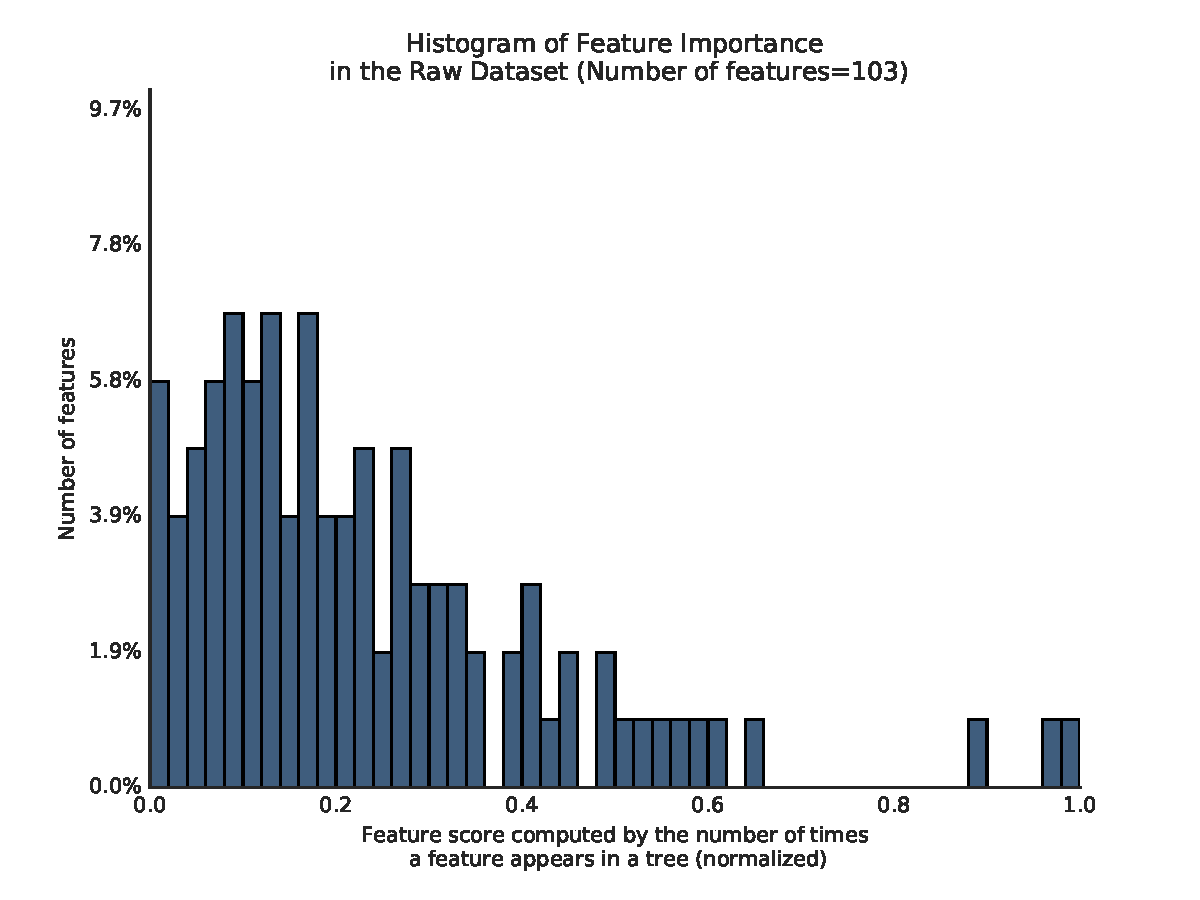
\includegraphics[width=\textwidth]{ch04/fi/fi_yeast_base}
        \caption{Yeast}
        \label{results:fi_yeast_base}
    \end{subfigure}
    ~ %add desired spacing between images, e. g. ~, \quad, \qquad, \hfill etc. 
      %(or a blank line to force the subfigure onto a new line)
    \begin{subfigure}[b]{0.45\textwidth}
        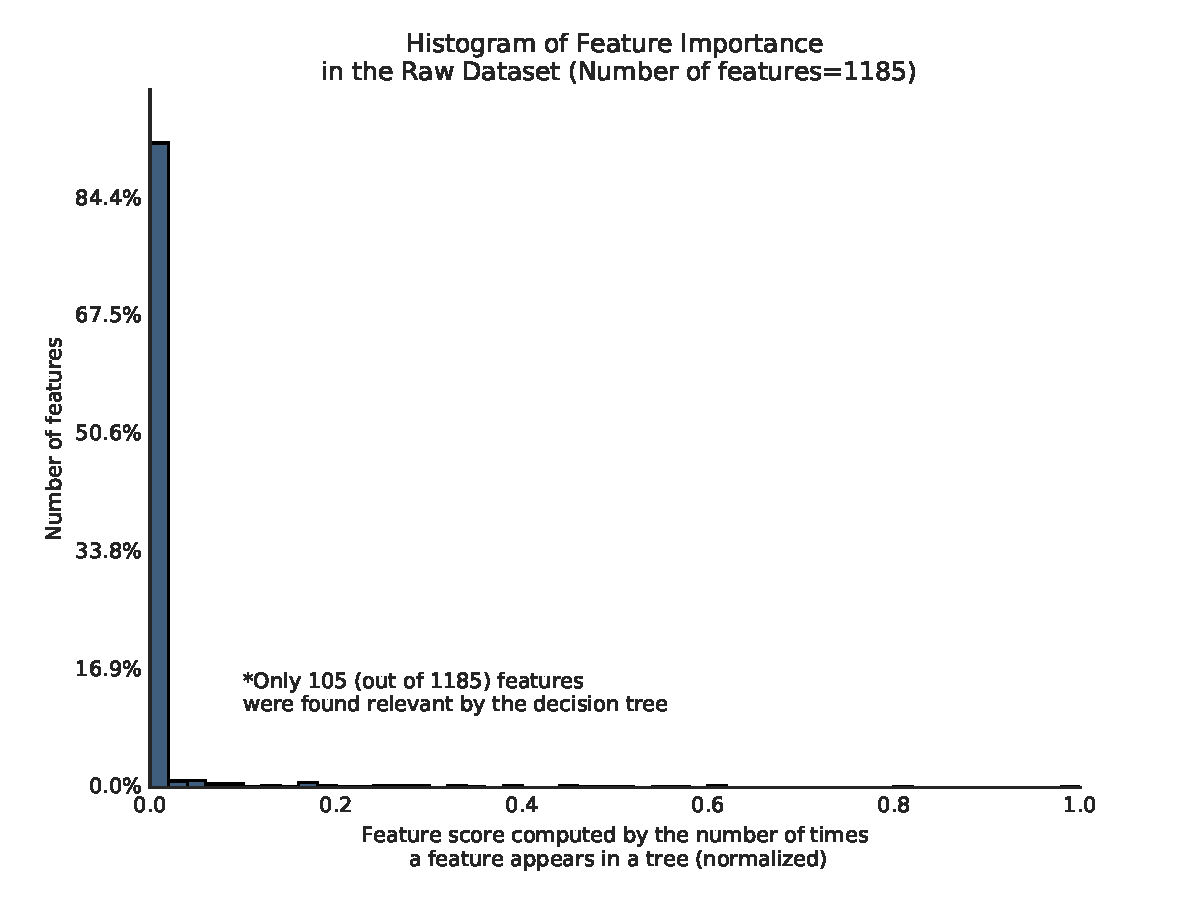
\includegraphics[width=\textwidth]{ch04/fi/fi_genbase_base}
        \caption{Genbase}
        \label{results:fi_genbase_base}
    \end{subfigure}
    \caption{Feature importance histogram for the raw data in both datasets}
    \label{results:fi_base}
\end{figure}

\begin{figure}[h!]
    \centering
    \begin{subfigure}[b]{0.45\textwidth}
        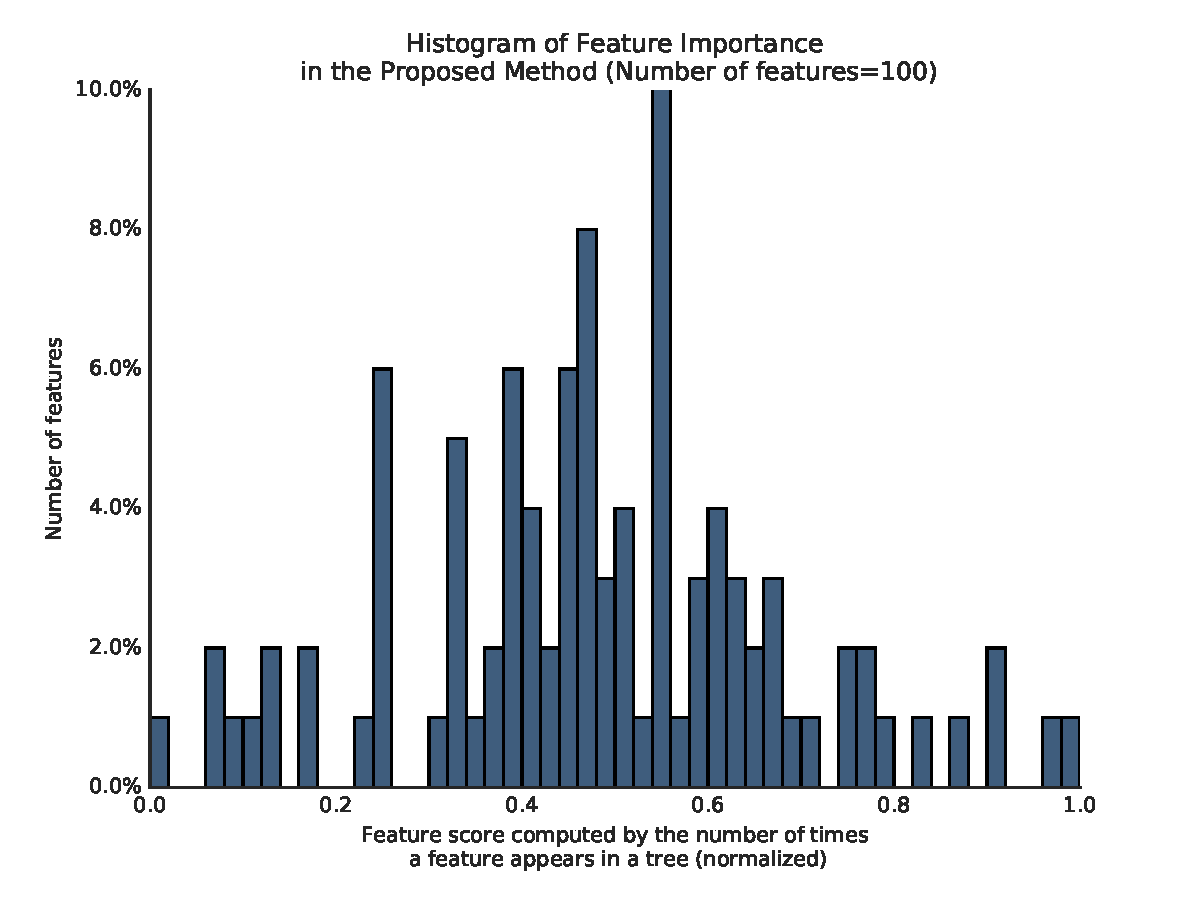
\includegraphics[width=\textwidth]{ch04/fi/fi_yeast_100}
        \caption{Number of features: $100$}
        \label{results:fi_yeast_100}
    \end{subfigure}
    ~ %add desired spacing between images, e. g. ~, \quad, \qquad, \hfill etc. 
      %(or a blank line to force the subfigure onto a new line)
    \begin{subfigure}[b]{0.45\textwidth}
        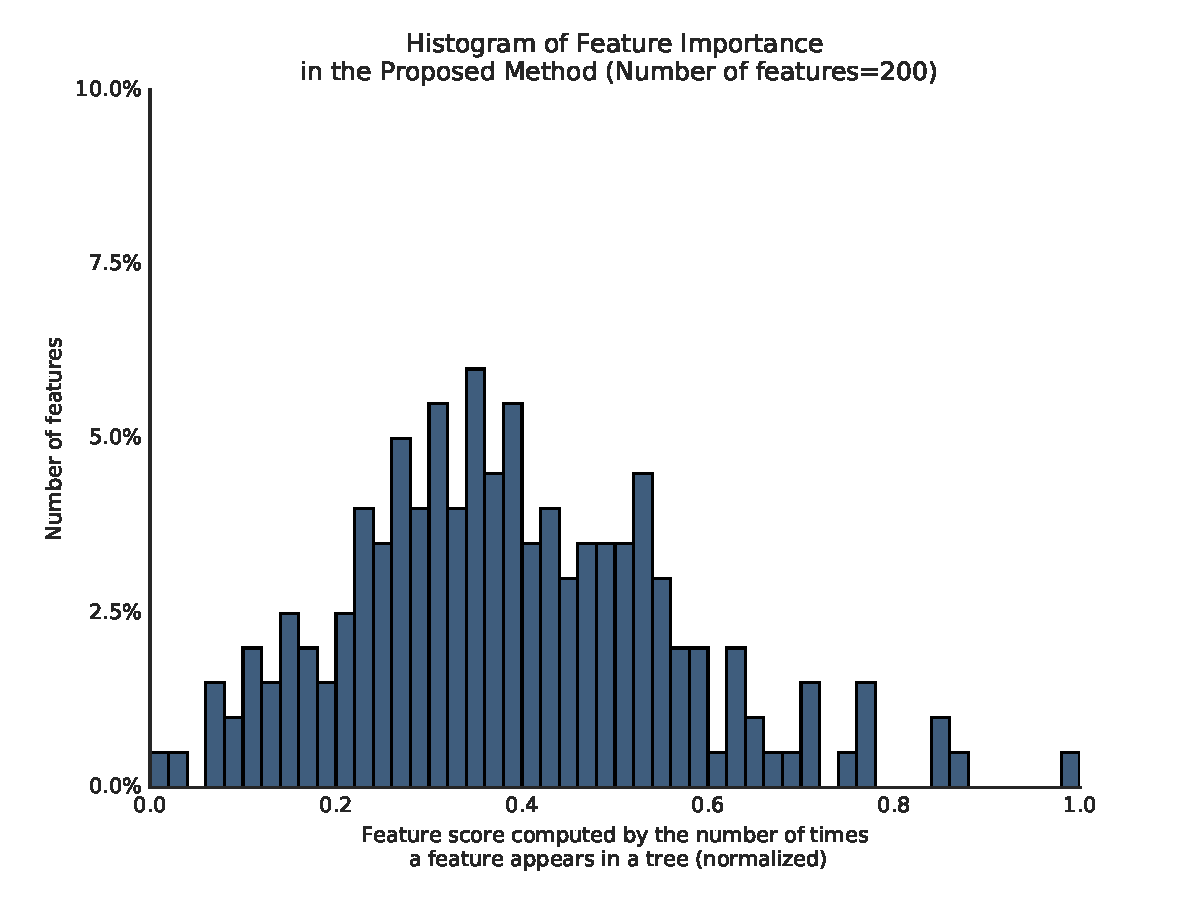
\includegraphics[width=\textwidth]{ch04/fi/fi_yeast_200}
        \caption{Number of features: $200$}
        \label{results:fi_yeast_200}
    \end{subfigure}
    ~ %add desired spacing between images, e. g. ~, \quad, \qquad, \hfill etc. 
      %(or a blank line to force the subfigure onto a new line)
    \begin{subfigure}[b]{0.45\textwidth}
        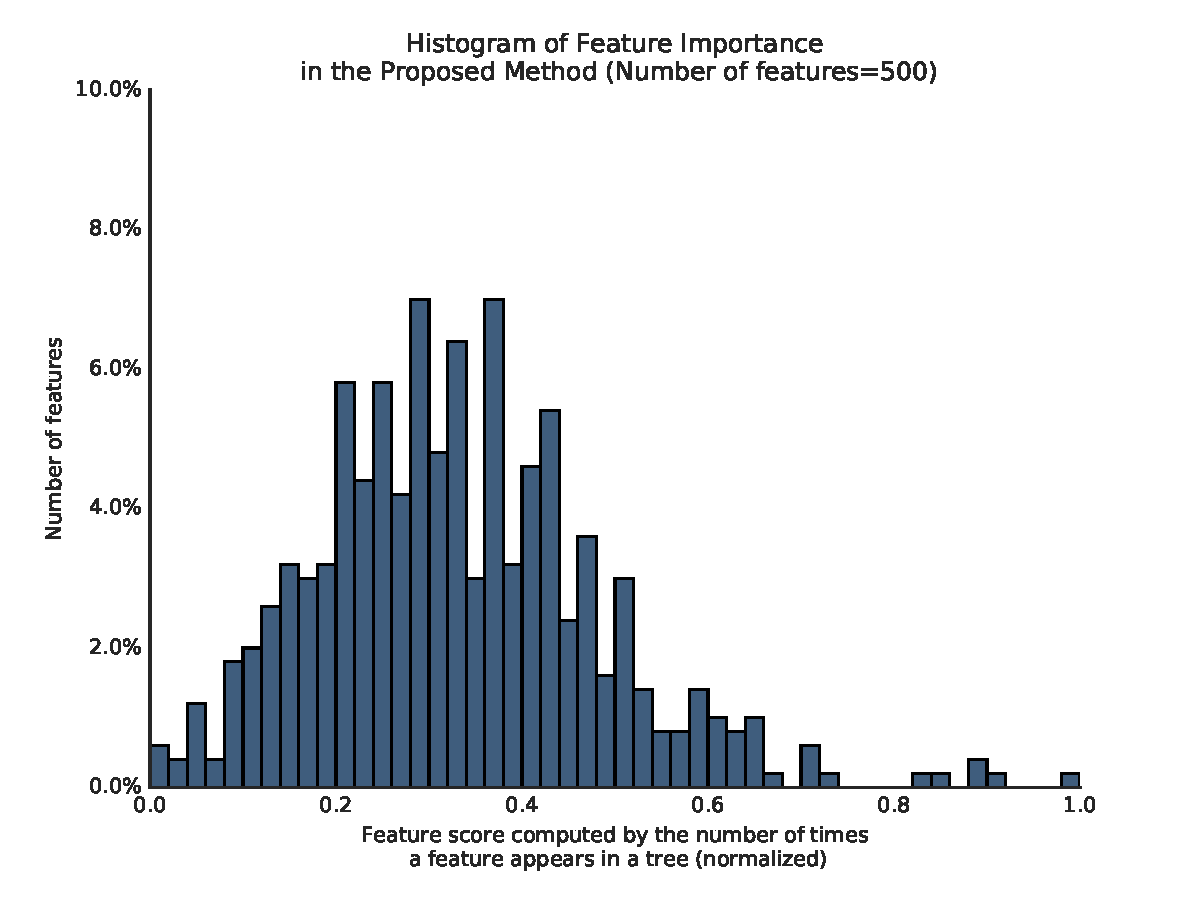
\includegraphics[width=\textwidth]{ch04/fi/fi_yeast_500}
        \caption{Number of features: $500$}
        \label{results:fi_yeast_500}
    \end{subfigure}
    ~ %add desired spacing between images, e. g. ~, \quad, \qquad, \hfill etc. 
      %(or a blank line to force the subfigure onto a new line)
    \begin{subfigure}[b]{0.45\textwidth}
        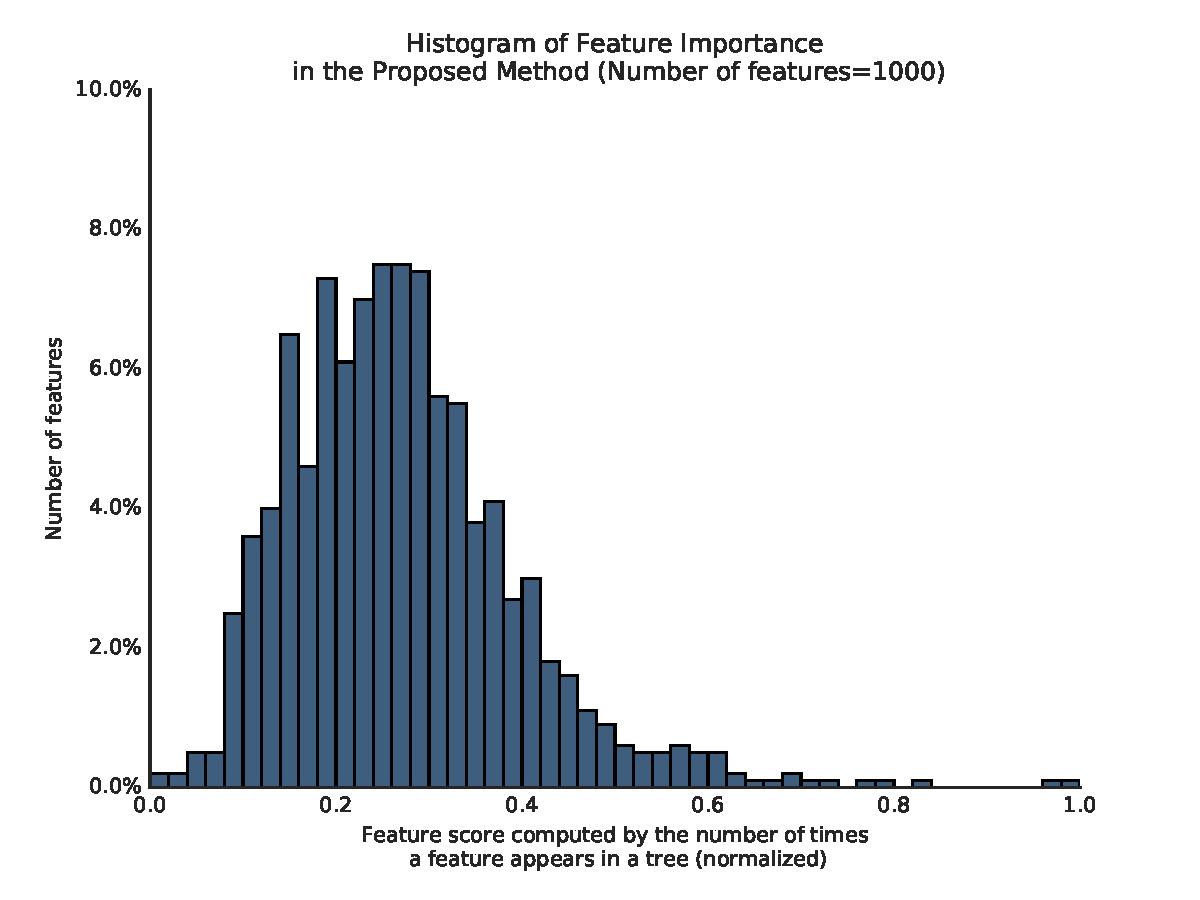
\includegraphics[width=\textwidth]{ch04/fi/fi_yeast_1000}
        \caption{Number of features: $1000$}
        \label{results:fi_yeast_1000}
    \end{subfigure}
    \caption{Feature importance histogram for the extracted features in Yeast}
    \label{results:fi_yeast}
\end{figure}

\paragraph{Yeast} The raw features tend to produce a left-leaning histogram
as shown in Figure \ref{results:fi_yeast_base}.  On the other hand, the score
distribution for the extracted features in Figure \ref{results:fi_yeast} have
moved into a higher range of scores. Interestingly, peaks are more noticeable
in lower dimensions, suggesting that relevant features are being extracted
while leaving others trivial. For higher dimensions, the distribution becomes
smoother. 

\begin{figure}[t]
    \centering
    \begin{subfigure}[b]{0.45\textwidth}
        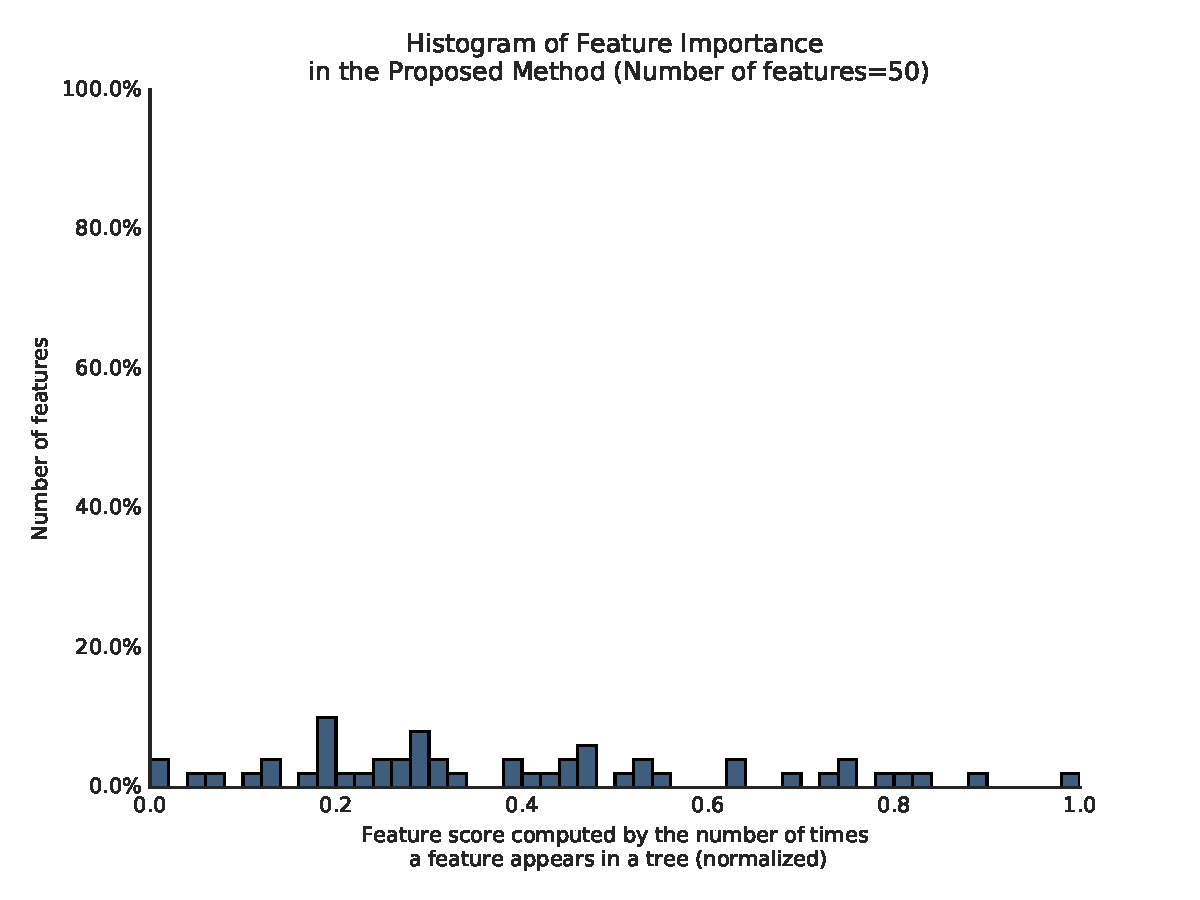
\includegraphics[width=\textwidth]{ch04/fi/fi_genbase_50}
        \caption{Number of features: $50$}
        \label{results:fi_genbase_50}
    \end{subfigure}
    ~ %add desired spacing between images, e. g. ~, \quad, \qquad, \hfill etc. 
      %(or a blank line to force the subfigure onto a new line)
    \begin{subfigure}[b]{0.45\textwidth}
        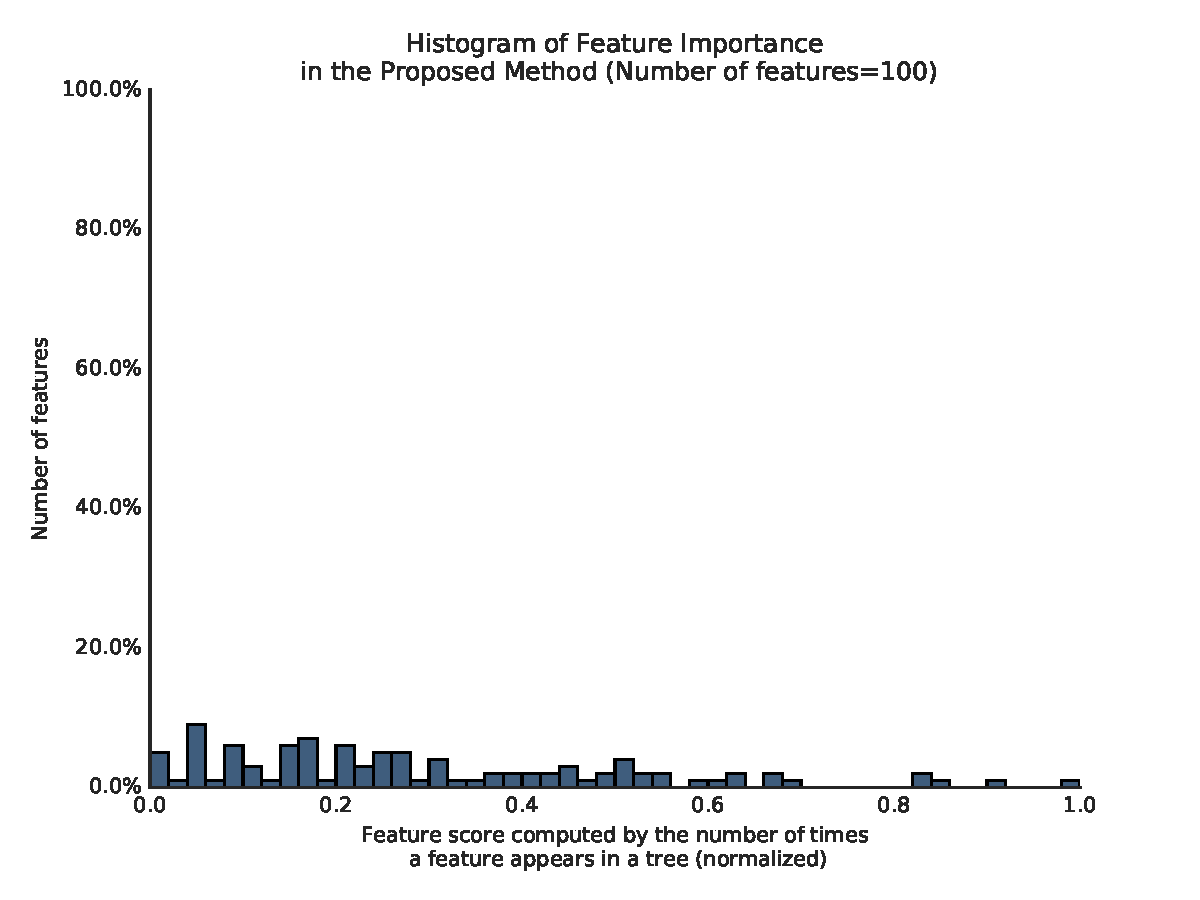
\includegraphics[width=\textwidth]{ch04/fi/fi_genbase_100}
        \caption{Number of features: $100$}
        \label{results:fi_genbase_100}
    \end{subfigure}
    ~ %add desired spacing between images, e. g. ~, \quad, \qquad, \hfill etc. 
      %(or a blank line to force the subfigure onto a new line)
    \begin{subfigure}[b]{0.45\textwidth}
        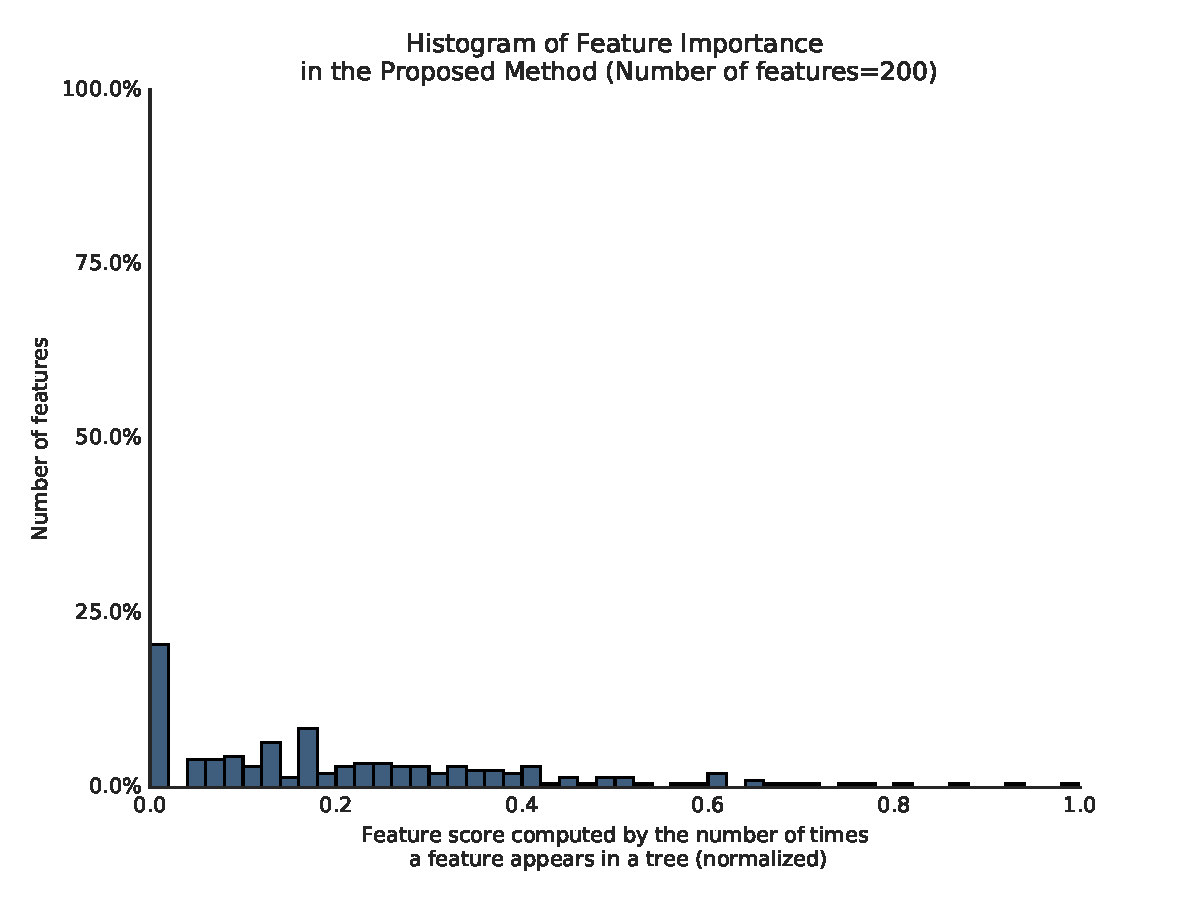
\includegraphics[width=\textwidth]{ch04/fi/fi_genbase_200}
        \caption{Number of features: $200$}
        \label{results:fi_genbase_200}
    \end{subfigure}
    ~ %add desired spacing between images, e. g. ~, \quad, \qquad, \hfill etc. 
      %(or a blank line to force the subfigure onto a new line)
    \begin{subfigure}[b]{0.45\textwidth}
        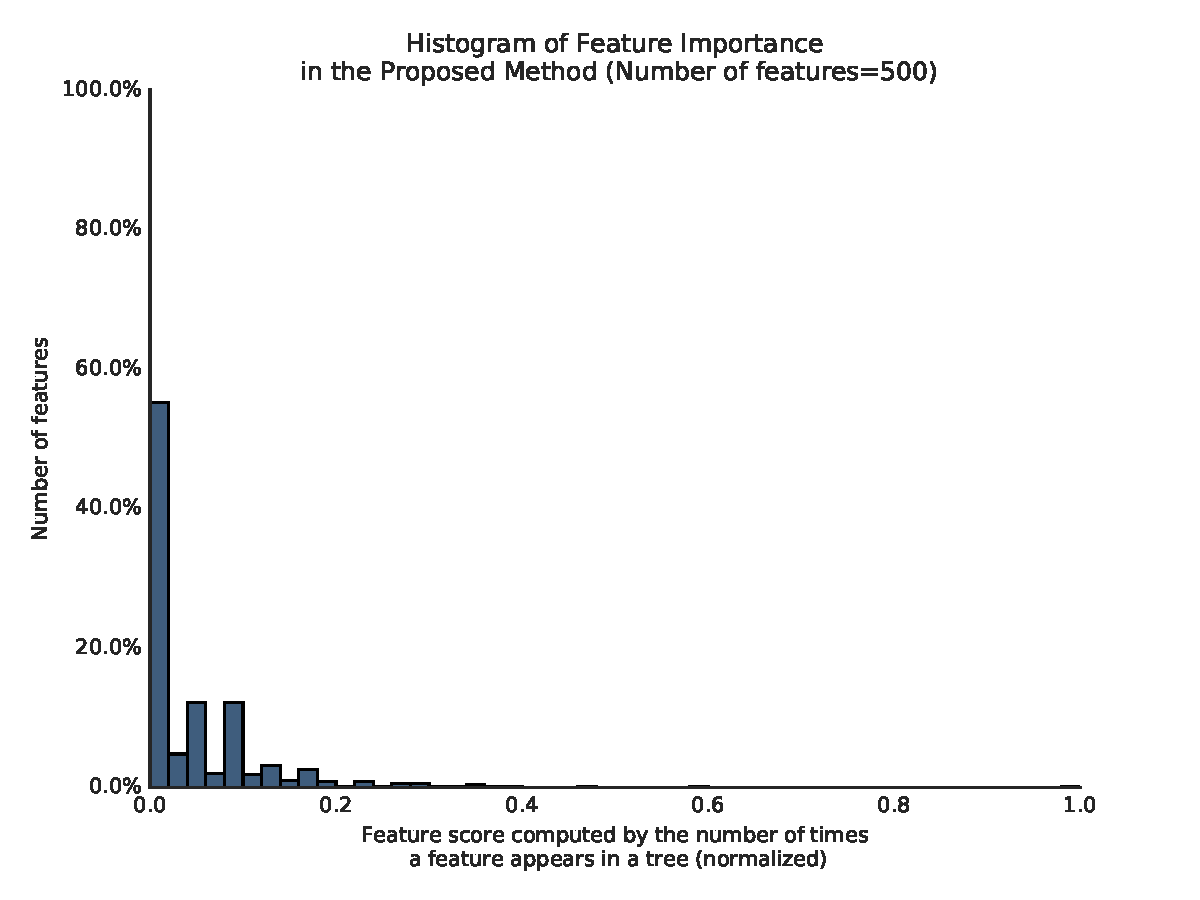
\includegraphics[width=\textwidth]{ch04/fi/fi_genbase_500}
        \caption{Number of features: $500$}
        \label{results:fi_genbase_500}
    \end{subfigure}
    \caption{Feature importance histogram for the extracted features in Genbase}
    \label{results:fi_genbase}
\end{figure}

\paragraph{Genbase} The histogram from \ref{results:fi_genbase_base} shows a
large number of the original feature set deemed irrelevant by the
decision-tree, as evidenced by the tall spike in the $0.0$ range. This suggests
that the features render the classification task more challenging. Compared
with the extracted features' scores in Figure \ref{results:fi_genbase}, the
distribution consists of more relevant features. The spike observed from the
raw inputs is not evident anymore (except in Fig.
\ref{results:fi_genbase_500}).\\

\par In summary, this experiment enables us to qualitatively observe how the
proposed method affects feature importance.  It is assumed that relevant
features boost classification, therefore helpful optimizing this
characteristic. By comparing feature score distribution across the whole
dataset, we can gauge feature relevance. From the experimental results, the
proposed method demonstrates the ability to extract more relevant features: the
score distribution of the new representations lie on the higher range in
contrast to the raw input. Next, we will investigate if feature relevance
indeed translates to better classification performance by measuring the quality
of the protein function prediction model.

\newpage
\section{Measuring model quality}
\label{ModelQuality}

\par This experiment enables us to gauge model performance in the two datasets.
Receiver operating characteristic (ROC) and precision-recall (PR) curves will
be drawn to accomplish this task. The ROC curve describes the sensitivity (true
positive rate) of the model as a function of its specificity (false positive
rate)\footnote[2]{In practice, we plot against $(1-\text{specificity})$} whereas
the PR curve illustrates the tradeoff between precision and recall for
different cutoff points. For both curves, a micro-average of all labels
will be plotted together with five (5) random classes in the labelset.

\begin{figure}[t]
    \centering
    \begin{subfigure}[b]{0.45\textwidth}
        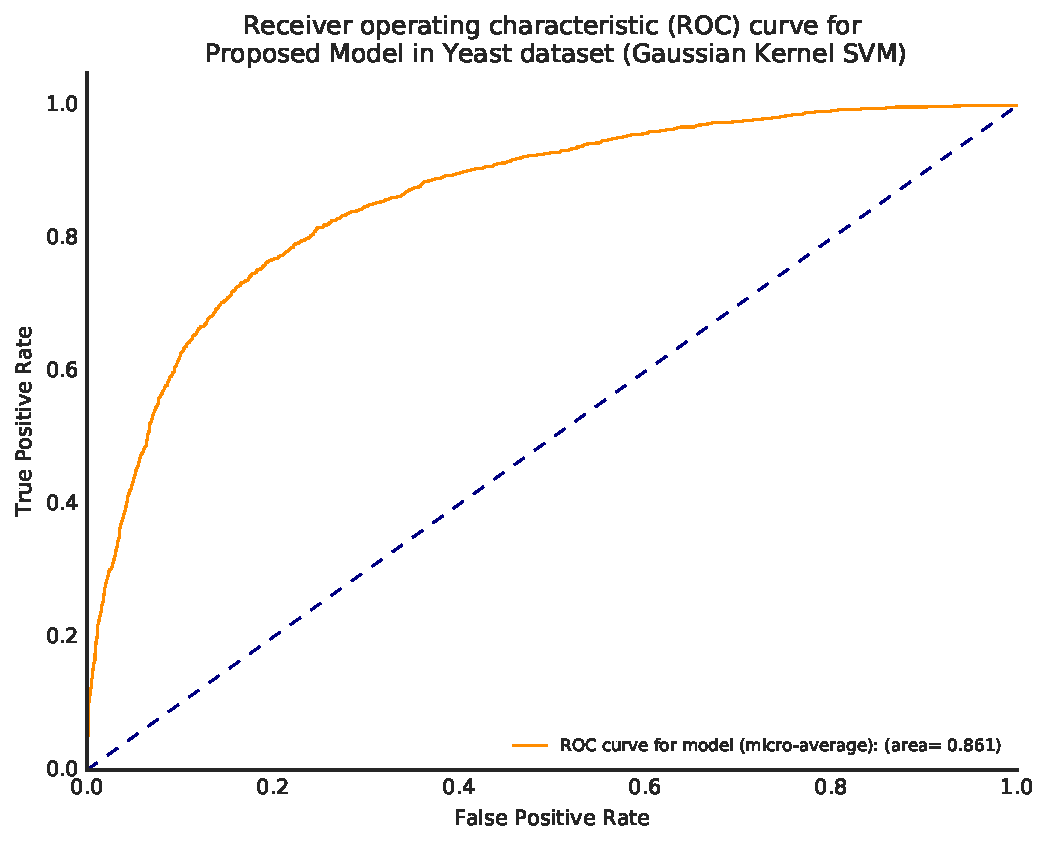
\includegraphics[width=\textwidth]{ch04/roc/roc_yeast_main}
        \caption{Micro-averaged across all labels}
        \label{results:roc_yeast_main}
    \end{subfigure}
    ~ %add desired spacing between images, e. g. ~, \quad, \qquad, \hfill etc. 
      %(or a blank line to force the subfigure onto a new line)
    \begin{subfigure}[b]{0.45\textwidth}
        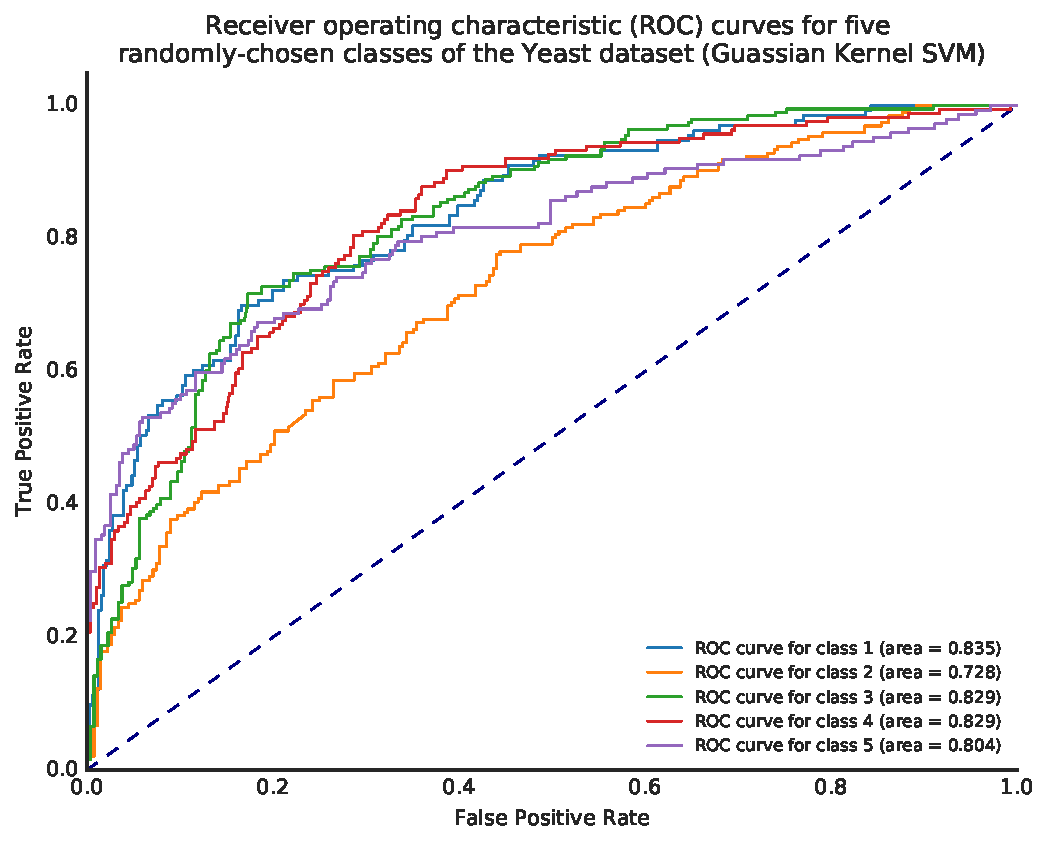
\includegraphics[width=\textwidth]{ch04/roc/roc_yeast_multiclass}
        \caption{Individual curves for five random labels}
        \label{results:roc_yeast_multiclass}
    \end{subfigure}
    \caption{Receiver Operating Characteristic (ROC) curves for the Yeast
    Dataset}
    \label{results:roc_yeast}
\end{figure}


\begin{figure}[t]
    \centering
    \begin{subfigure}[b]{0.45\textwidth}
        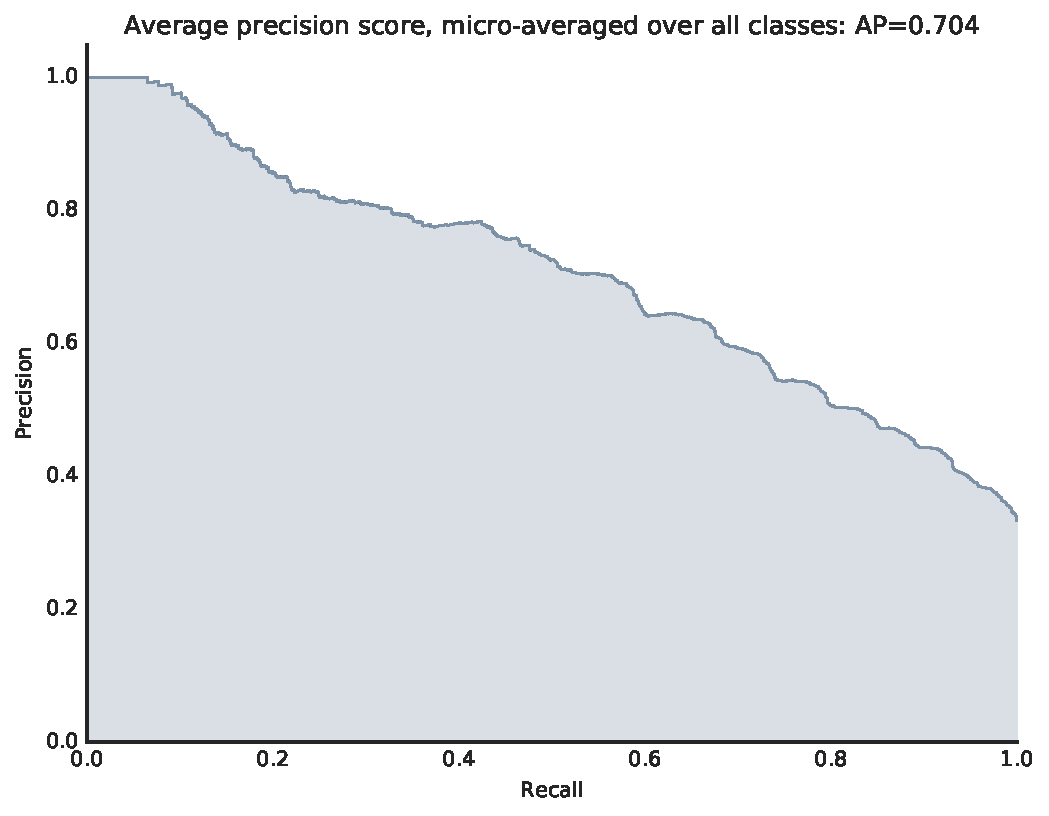
\includegraphics[width=\textwidth]{ch04/pr/pr_yeast_main}
        \caption{Micro-averaged across all labels}
        \label{results:pr_yeast_main}
    \end{subfigure}
    ~ %add desired spacing between images, e. g. ~, \quad, \qquad, \hfill etc. 
      %(or a blank line to force the subfigure onto a new line)
    \begin{subfigure}[b]{0.45\textwidth}
        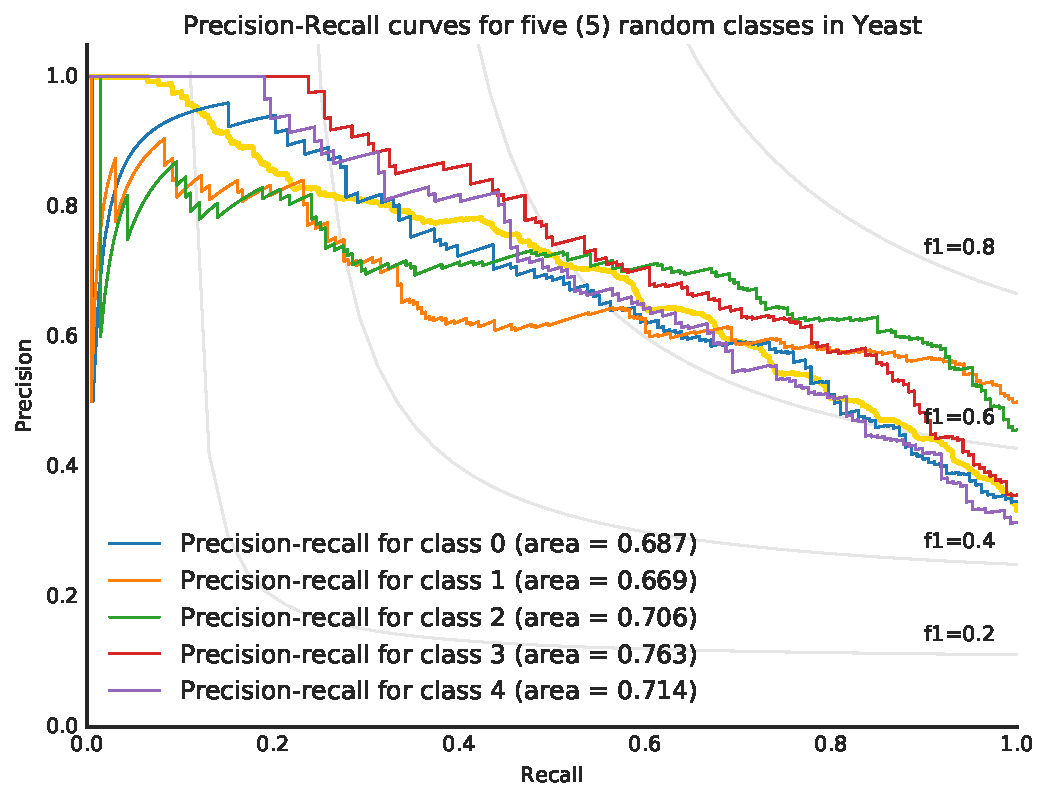
\includegraphics[width=\textwidth]{ch04/pr/pr_yeast_multi}
        \caption{Individual curves for five random labels}
        \label{results:pr_yeast_multi}
    \end{subfigure}
    \caption{Precision-Recall (PR) curves for the Yeast dataset}
    \label{results:pr_yeast}
\end{figure}

\paragraph{Yeast} Figure \ref{results:roc_yeast_main} shows that the model has
better performance than the baseline, given its large area under the curve
(i.e., $0.861$). In addition, the curves on Fig.
\ref{results:roc_yeast_multiclass} also have relatively large areas under it,
indicating that the quality is well-distributed to different labels. Lastly,
the PR curves in Fig.  \ref{results:pr_yeast} show an estimated F-score in the
range of $0.5$ to $0.7$, and can still be improved by tuning the
hyperparameters.

\paragraph{Genbase} For this dataset, the model tends to perform well as
evidenced by the $0.995$ performance in Figure \ref{results:roc_genbase_main}.
This is also well-distributed to different classes as evidenced by Fig.
\ref{results:roc_genbase_multiclass}. Lastly, the PR-curves show conformation to
this quality, showing a good score even for different classes.  \\ 


\begin{figure}[t]
    \centering
    \begin{subfigure}[b]{0.45\textwidth}
        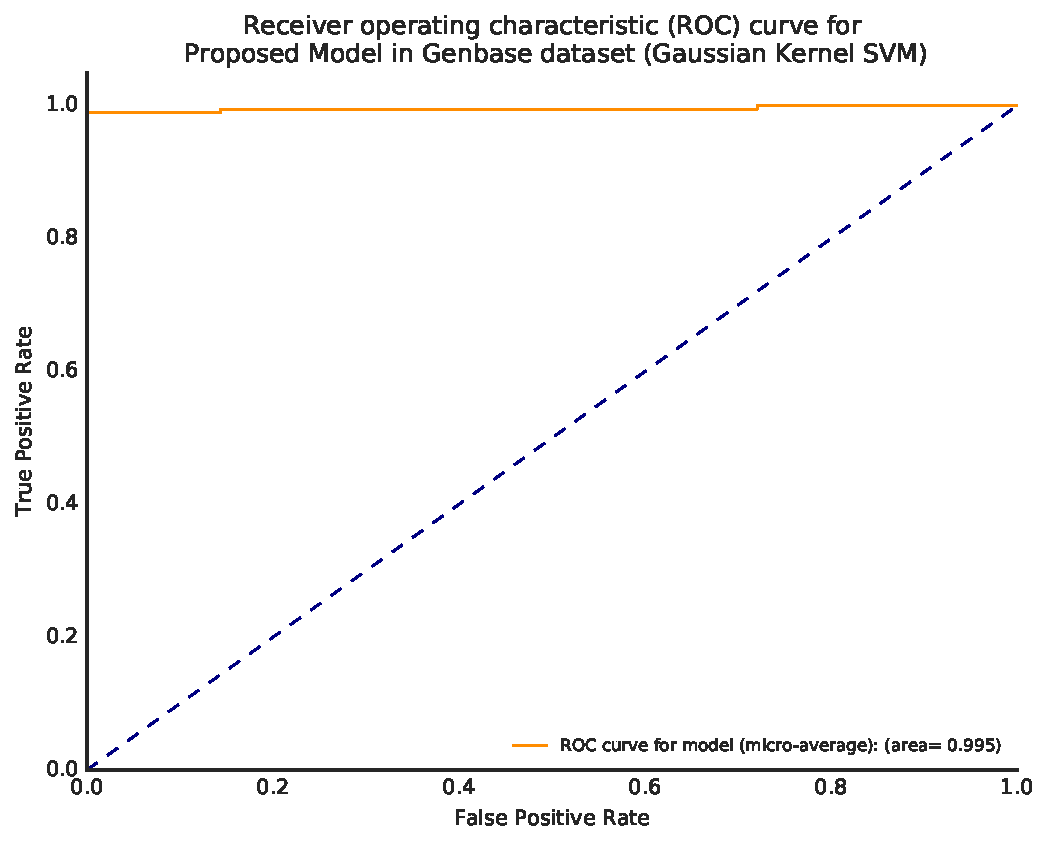
\includegraphics[width=\textwidth]{ch04/roc/roc_genbase_main}
        \caption{Micro-averaged across all labels}
        \label{results:roc_genbase_main}
    \end{subfigure}
    ~ %add desired spacing between images, e. g. ~, \quad, \qquad, \hfill etc. 
      %(or a blank line to force the subfigure onto a new line)
    \begin{subfigure}[b]{0.45\textwidth}
        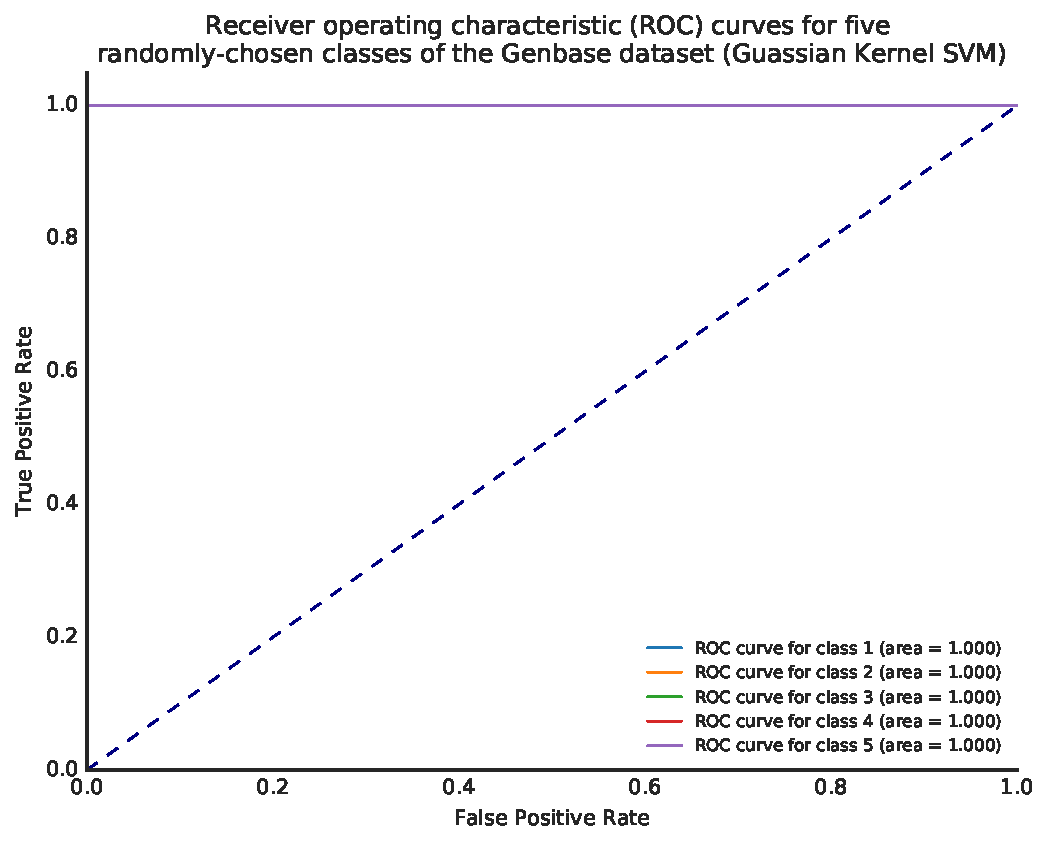
\includegraphics[width=\textwidth]{ch04/roc/roc_genbase_multiclass}
        \caption{Individual curves for five random labels}
        \label{results:roc_genbase_multiclass}
    \end{subfigure}
    \caption{Receiver Operating Characteristic (ROC) curves for the Genbase
    Dataset}
    \label{results:roc_genbase}
\end{figure}


\begin{figure}[t]
    \centering
    \begin{subfigure}[b]{0.45\textwidth}
        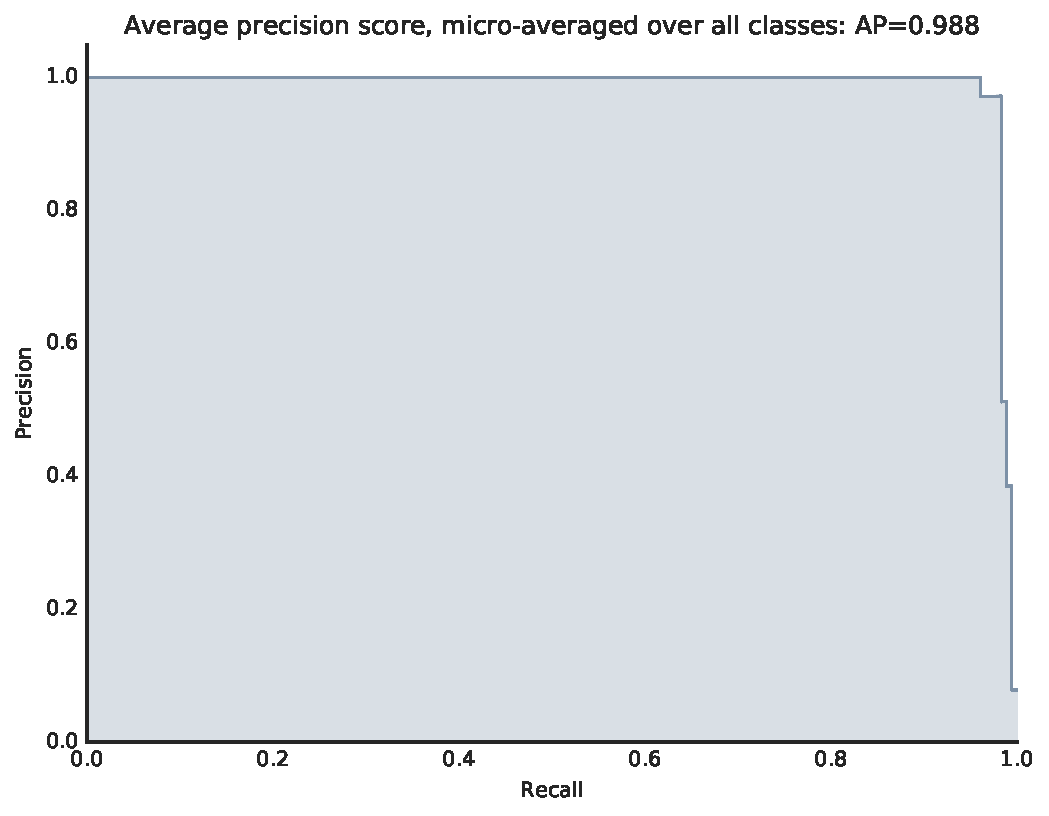
\includegraphics[width=\textwidth]{ch04/pr/pr_genbase_main}
        \caption{Micro-averaged across all labels}
        \label{results:pr_genbase_main}
    \end{subfigure}
    ~ %add desired spacing between images, e. g. ~, \quad, \qquad, \hfill etc. 
      %(or a blank line to force the subfigure onto a new line)
    \begin{subfigure}[b]{0.45\textwidth}
        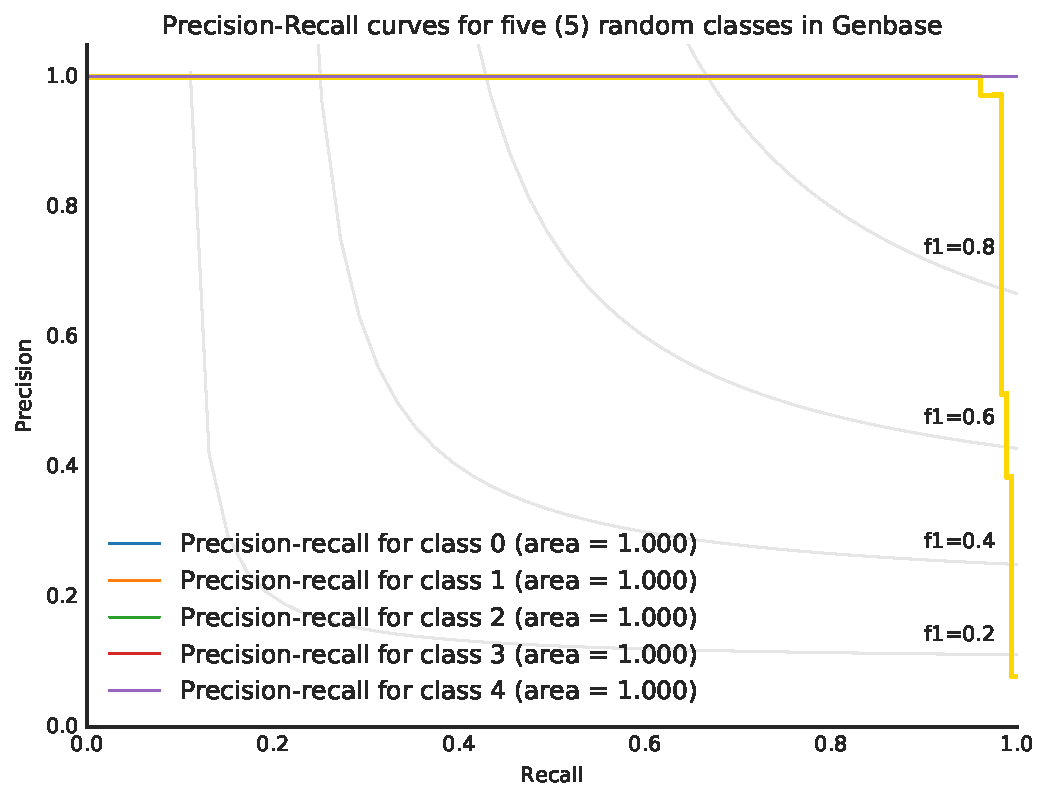
\includegraphics[width=\textwidth]{ch04/pr/pr_genbase_multi}
        \caption{Individual curves for five random labels}
        \label{results:pr_genbase_multi}
    \end{subfigure}
    \caption{Precision-Recall (PR) curves for the Genbase dataset}
    \label{results:pr_genbase}
\end{figure}

\par Lastly, Table \ref{results:pr_table} gives the precision and recall
measurements for the model using two different SVM kernels and three averaging
methods. It is evident that using the Gaussian kernel for SVM works in favor to
improve model performance. In addition, the results are relatively decent and
can still be improved by hyperparameter tuning.

\begin{table}[!ht]
    \centering
    \caption{Average precision and recall for both datasets}
    \label{results:pr_table}
    \begin{tabular}{@{}lrllcll@{}}
    \toprule
     &         & \multicolumn{5}{c}{Dataset}                             \\ \cmidrule{3-7}
     &         & \multicolumn{2}{c}{Yeast} &\phantom{abc} & \multicolumn{2}{c}{Genbase} \\ \cmidrule{3-4} \cmidrule{6-7}
     &                      & Linear     & Gaussian  && Linear    & Gaussian  \\ \midrule
\multicolumn{2}{l}{Precision} \\
     & \textit{micro}       & 0.538191   & 0.639692  &&  0.988006 & 0.973023  \\
     & \textit{macro}       & 0.569659   & 0.648473  &&  0.980438 & 0.988342  \\
     & \textit{samples}     & 0.545558   & 0.648483  &&  0.994149 & 0.982895  \\
\multicolumn{2}{l}{Recall} \\
     & \textit{micro}       & 0.577003   & 0.618419  &&  0.986286 & 1.000000  \\
     & \textit{macro}       & 0.577003   & 0.618419  &&  0.986286 & 1.000000  \\
     & \textit{samples}     & 0.583777   & 0.636325  &&  0.991726 & 1.000000  \\ \bottomrule
    \end{tabular}
\end{table}


\par In summary, the ROC and PR curves gave insights on model performance for
the two datasets. From the experimental results, the proposed model delivered
higher performance compared to the baseline\textemdash  defined as a classifier
with area under ROC of $0.5$. In addition, the PR curves also demonstrated a
good precision-recall tradeoff for both datasets. However, model quality cannot
easily be judged in isolation. For the next set of experiments, we will put
model performance into context by benchmarking it against other techniques in
literature. 

\section{Comparison to other models}
\label{Benchmarking}

\par In this section, the proposed model will be compared to other works in
literature. The existing works follow the same pipeline for protein function
prediction\textemdash extract features from data, then classify with the
extracted features:

\begin{itemize}
    \item \cite{wang2013protein} applied principal component
    analysis (PCA) to reduce the dimensions of protein data from $353$ to
    $204$. 
    \item \cite{chicco2014deep} used a deep autoencoder with two-layers
    to predict the protein functions of \textit{B.taurus} and \textit{G.
    gallus}. 
    \item \cite{miranda2017feature} implemented a stacked denoising
    autoencoder to obtain robust features from raw data to predict protein
    functions.  
\end{itemize}

\par In addition, we will also compare against a baseline model without feature
extraction. All features, extracted or not, will be trained on a
binary-relevance SVM for classification with both gaussian and linear kernels.
The trained model then predicts the samples from a held-out test set.  The
entire pipeline will run for ten (10) trials with the mean and standard
deviation reported. Tables \ref{results:yeast_svm} to \ref{results:genbase_lsvm}
show the outcome for the two datasets using different SVM kernels.

\par The top performer is highlighted in bold font for each criteria: the
highest value for AUROC and F-score and the lowest for Hamming loss. Overall,
the proposed method outperformed all other techniques in literature including
the baseline. However, to fully assess our model's performance, statistical
tests of significance are implemented.

\subsection{Statistical tests of significance}

To assess if the performance of the proposed model is significant against other
techniques, two statistical tests were employed: Friedman's test
and a post-hoc Nemenyi test. The Friedman's test determines if the results across all
methods are significantly different. If difference is detected, then a post-hoc
Nemenyi test checks for significant difference in each method against the proposed
model \footnote[2]{Friedman's test asks the following question: are methods A,
B, C different from one another? If they are, then a post-hoc Nemenyi test will
ask: is method A significantly different to method B? to method C? and so on.}.
These tests were recommended by \cite{demsar2006statistical}  and was patterned
from most literature reviews in multilabel learning
(\cite{madjarov2012extensive, zhang2014review}). 

\par For the Friedman's test, the null hypothesis $H_{0}$ states that there is no
significant difference across all methods. Comparing the computed
$\chi^{2}$ statistic and $p$-value, we can reject $H_{0}$ at different
confidence level $\alpha$ as summarized in Table
\ref{results:friedman}. At the same time, the test can be performed at
different levels of comparison: (i) across each dataset and classifier, (ii)
across datasets, (iii) overall. From the test results, it is evident that
there is significant difference among the models' performance.Thus we can
proceed to a post-hoc test.

\par Because all datasets passed the Friedman's test, a post-hoc Nemenyi test
can be implemented to check the proposed model's performance against other
methods. Here, the null hypothesis $H_{0}$ states that there is no
significant difference between two methods A and B. Table
\ref{results:nemenyi} shows the results when comparing each method across
datasets and overall. 

\begin{table}[!ht]
    \footnotesize
    \centering
    \caption{Results for the Yeast Dataset using SVM with Gaussian Kernel}
    \label{results:yeast_svm}
    \begin{threeparttable}
    \begin{tabular}{@{}rrlllll@{}}
    \toprule
    && \multicolumn{5}{c}{Prediction Model} \\ \cmidrule{3-7}
    \multicolumn{2}{r}{Metrics}               & Baseline                & Wang, 2013 & Chicco, 2014 & Miranda, 2017 & Proposed            \\ \midrule
\multicolumn{2}{l}{Area ROC} \\
                    & \textit{micro}            & $0.6668 \pm 0.0031$ & $0.6559 \pm 0.0020$ & $0.6430 \pm 0.0012$ & $0.6679 \pm 0.0025$ & $\mathbf{0.7320 \pm 0.0021} $ \\
                     & \textit{macro}            & $0.6548 \pm 0.0031$ & $0.6590 \pm 0.0024$ & $\mathbf{0.6624 \pm 0.0011}$ & $0.6484 \pm 0.0022$ & $0.6455 \pm 0.0018 $ \\
                     & \textit{samples}            & $0.6700 \pm 0.0032$ & $0.6559 \pm 0.0019$ & $0.6443 \pm 0.0011$ & $0.6569 \pm 0.0026$ & $\mathbf{0.7433 \pm 0.0040} $ \\
\multicolumn{2}{l}{F-score} \\
                    & \textit{micro}            & $0.5483 \pm 0.0041$ & $0.5381 \pm 0.0023$ & $0.5304 \pm 0.0014$ & $0.5792 \pm 0.0028$ & $\mathbf{0.6289 \pm 0.0024} $ \\
                     & \textit{macro}            & $0.5970 \pm 0.0035$ & $0.6033 \pm 0.0024$ & $0.5896 \pm 0.0011$ & $0.6132 \pm 0.0023$ & $\mathbf{0.6299 \pm 0.0024} $ \\
                     & \textit{samples}            & $0.5359 \pm 0.0032$ & $0.5242 \pm 0.0022$ & $0.5171 \pm 0.0014$ & $0.5720 \pm 0.0034$ & $\mathbf{0.6086 \pm 0.0038} $ \\ 
\multicolumn{2}{l}{Hamm. Loss}            & $0.3222 \pm 0.0021$ & $0.3430 \pm 0.0018$ & $0.3535 \pm 0.0011$ & $0.2310 \pm 0.0031$ & $\mathbf{0.2241 \pm 0.0019}$ \\
\bottomrule
    \end{tabular}
    \begin{tablenotes}
        \item SVM Hyperparameters for Proposed Model: $C=1.000$, $\gamma=1.67e-3$
    \end{tablenotes}
    \end{threeparttable}
\end{table}

\begin{table}[t]
    \footnotesize
    \centering
    \caption{Results for the Yeast Dataset using SVM with Linear Kernel}
    \label{results:yeast_lsvm_main}
    \begin{threeparttable}
    \begin{tabular}{@{}lllllll@{}}
    \toprule
    \multicolumn{2}{l}{Metrics}      & Base                 & PCA                  & AE                  & SdAE          & Proposed      \\ \midrule
    H     & \textit{--}               & $0.3507 \pm 0.0012$  & $0.3619  \pm 0.0021$ & $0.3739 \pm 0.0005$ & $0.3170 \pm 0.0036$ & $\mathbf{0.2794 \pm 0.0053}$ \\
    A     & \textit{mi}              & $0.6504 \pm 0.0021$  & $0.6465 \pm 0.0022$  & $0.6287 \pm 0.0005$ & $0.6425 \pm 0.0022$ & $\mathbf{0.6802 \pm 0.0071}$ \\
          & \textit{ma}              & $0.6507 \pm 0.0016$  & $\mathbf{0.6548 \pm 0.0016}$  & $0.6524 \pm 0.0009$ & $0.6099 \pm 0.0013$ & $0.6012 \pm 0.0072$ \\
          & \textit{sp}              & $0.6525 \pm 0.0022$  & $0.6499 \pm 0.0023$  & $0.6299 \pm 0.0005$ & $0.6471 \pm 0.0019$ & $\mathbf{0.6851 \pm 0.0079}$ \\
    F     & \textit{mi}              & $0.5330 \pm 0.0032$  & $0.5305 \pm 0.0025$  & $0.5173 \pm 0.0006$ & $0.5445 \pm 0.0024$ & $\mathbf{0.5569 \pm 0.0097}$ \\
          & \textit{ma}              & $0.5913 \pm 0.0031$  & $\mathbf{0.6023 \pm 0.0019}$  & $0.5816 \pm 0.0006$ & $0.5779 \pm 0.0019$ & $0.5709 \pm 0.0094$ \\
          & \textit{sp}              & $0.5223 \pm 0.0031$  & $0.5217 \pm 0.0027$  & $0.5101 \pm 0.0008$ & $0.5302 \pm 0.0020$ & $\mathbf{0.5354 \pm 0.0107}$ \\ \bottomrule
    \end{tabular}
    \begin{tablenotes}
      \item SVM Hyperparameters for Proposed Model: $C=3.594$
    \end{tablenotes}
   \end{threeparttable}
\end{table}


\begin{table}[h!]
    \footnotesize
    \centering
    \caption{Results for the Genbase Dataset using SVM with Gaussian Kernel}
    \label{results:genbase_svm}
    \begin{threeparttable}
    \begin{tabular}{@{}rrlllll@{}}
    \toprule
    && \multicolumn{5}{c}{Prediction Model} \\ \cmidrule{3-7}
    \multicolumn{2}{r}{Metrics}               & Baseline                & Wang, 2013 & Chicco, 2014 & Miranda, 2017 & Proposed            \\ \midrule
\multicolumn{2}{l}{Area ROC} \\
           & \textit{micro}       & $0.8563 \pm 0.0002$ & $0.9872 \pm 0.0001$ &
$0.9741 \pm 0.0098$ & $0.9872 \pm 0.0009$ & $\mathbf{0.9992 \pm 0.0000}$ \\
            & \textit{macro}       & $0.6706 \pm 0.0004$ & $0.9928 \pm 0.0002$
            & $0.9786 \pm 0.0106$ & $0.9834 \pm 0.0009$ & $\mathbf{0.9996 \pm
            0.0000}$ \\
            & \textit{samples}       & $0.6129 \pm 0.0003$ & $0.9503 \pm
0.0001$ & $0.9756 \pm 0.0097$ & $0.9875 \pm 0.0007$ & $\mathbf{0.9992 \pm
0.0000}$ \\
\multicolumn{2}{l}{F-score} \\
           & \textit{micro}       & $0.6706 \pm 0.0003$ & $0.8872 \pm 0.0008$ &
$0.7846 \pm 0.0865$ & $0.9619 \pm 0.0109$ & $\mathbf{0.9863 \pm 0.0070}$ \\
            & \textit{macro}       & $0.7159 \pm 0.0005$ & $0.9503 \pm 0.0002$
            & $0.8922 \pm 0.0400$ & $0.9640 \pm 0.0061$ & $\mathbf{0.9919 \pm
            0.0020}$ \\
            & \textit{samples}       & $0.7603 \pm 0.0001$ & $0.9282 \pm 0.0004$ & $0.8098 \pm 0.0945$ & $0.9699 \pm 0.0080$ & $\mathbf{0.9886 \pm 0.0063}$ \\ 
    \multicolumn{2}{l}{Hamm. Loss} & $0.0407 \pm 0.0001$ & $0.0141 \pm 0.0021$
                                   & $0.0352 \pm 0.0168$ & $0.0045 \pm 0.0013$
                                   & $\mathbf{0.0016 \pm 0.0000}$ \\ \bottomrule
    \end{tabular}
    \begin{tablenotes}
        \item SVM Hyperparameters for Proposed Model: $C=1.000$, $\gamma=1.24e-3$
    \end{tablenotes}
    \end{threeparttable}
    \end{table}

\begin{table}[!ht]
    \footnotesize
    \centering
    \caption{Results for the Genbase Dataset using SVM with Linear Kernel}
    \label{results:genbase_lsvm}
    \begin{threeparttable}
        \begin{tabular}{@{}rrlllll@{}}
        \toprule
    && \multicolumn{5}{c}{Prediction Model} \\ \cmidrule{3-7}
    \multicolumn{2}{r}{Metrics}               & Baseline                & Wang, 2013 & Chicco, 2014 & Miranda, 2017 & Proposed            \\ \midrule
\multicolumn{2}{l}{Area ROC} \\
                   & \textit{micro}       & $0.9779 \pm 0.0079$ & $0.9782 \pm 0.0015$ & $0.9493 \pm 0.0165$ & $0.9926 \pm 0.0014$ & $\mathbf{0.9928 \pm 0.0019}$ \\
                    & \textit{macro}       & $0.9770 \pm 0.0010$ & $0.9876 \pm 0.0013$ & $0.9628 \pm 0.0151$ & $\mathbf{0.9936 \pm 0.0004}$ & $0.9929 \pm 0.0019$ \\
                    & \textit{samples}       & $0.9795 \pm 0.0015$ & $0.9796 \pm 0.0013$ & $0.9515 \pm 0.0165$ & $0.9948 \pm 0.0013$ & $\mathbf{0.9955 \pm 0.0010}$ \\
\multicolumn{2}{l}{F-score} \\
                   & \textit{micro}       & $0.7495 \pm 0.0023$ & $0.8074 \pm 0.0042$ & $0.6054 \pm 0.0884$ & $0.9671 \pm 0.0216$ & $\mathbf{0.9871 \pm 0.0034}$ \\
                    & \textit{macro}       & $0.8209 \pm 0.0081$ & $0.9198 \pm 0.0002$ & $0.7793 \pm 0.0581$ & $0.9757 \pm 0.0070$ & $\mathbf{0.9824 \pm 0.0033}$ \\
                    & \textit{samples}       & $0.8279 \pm 0.0088$ & $0.8474 \pm 0.0012$ & $0.6965 \pm 0.0711$ & $0.9732 \pm 0.0188$ & $\mathbf{0.9916 \pm 0.0022}$ \\ 
\multicolumn{2}{l}{Hamm. Loss}                & $0.0367 \pm 0.0041$ & $0.0263
\pm 0.0021$ & $0.0840 \pm 0.0309$ & $0.0038 \pm 0.0026$ & $\mathbf{0.0014 \pm
0.0004}$ \\ \bottomrule
        \end{tabular}
        \begin{tablenotes}
                \item SVM Hyperparameters for Proposed Model: $C=4.500$
        \end{tablenotes}
    \end{threeparttable}
    \end{table}


\par For the Yeast dataset, the proposed method's performance is not that
apparent against the $\textit{Baseline}$ and \cite{wang2013protein}, but are
significant against the two autoencoder models. For the Genbase dataset, the
proposed method's performance is not that significant against
\cite{miranda2017feature}, but are significant against all other techniques ($p
\leq 0.01$ and $p \leq 0.05$). Lastly, when accounting for overall performance,
the proposed method significantly performs better against other techniques in
literature ($p \leq 0.01$).

\par In summary, this set of experiments aims to determine how well the
proposed method performs against other techniques in literature. Test results
showed that the autoencoder with mutual competition performs significantly
better than the baseline and to other feature extraction methods. Overall, the
post-hoc Nemenyi test confirmed that the proposed model outperforms others in
the two classification tasks. This also showed that extracting features before
classification improves inference, as the model exceeds baseline performance.
Next, we will further test if the modifications to the basic autoencoder are
relevant by way of ablation. The proposed model will be built gradually,
adding one hyperparameter over the other to the basic autoencoder, while being
tested for AUROC.  

\begin{table}[t]
    \footnotesize
    \centering
    \caption{$p$-values for Friedman's test of significance}
    \label{results:friedman}
    \begin{threeparttable}
    \begin{tabular}{@{}llll@{}}
    \toprule
    Comparison                & $\chi^2$    & $p$-value       & Sig.\tnote{1}   \\ \midrule
    Yeast with Gaussian-SVM   & $13.257$    & $0.0101$        & **              \\
    Yeast with Linear-SVM     & $11.200$    & $0.0244$        & **              \\
    Genbase with Gaussian-SVM & $26.388$    & $2.642e-5$      & ***             \\
    Genbase with Linear-SVM   & $27.314$    & $1.717e-5$      & ***             \\ \cmidrule{1-4}
    Yeast                     & $18.400$    & $0.001031$      & ***             \\
    Genbase                   & $50.251$    & $3.201e-10$     & ***             \\ \cmidrule{1-4}
    Overall (all datasets)    & $47.335$    & $1.299e-09$     & ***             \\ \bottomrule
    \end{tabular}
    \begin{tablenotes}
        \item[1] Significance: * - $p \leq 0.1$, ** - $p \leq 0.05$, *** - $p \leq 0.01$
    \end{tablenotes}
    \end{threeparttable}
\end{table}

\begin{table}[t]
    \footnotesize
    \centering
    \caption{$p$-values from the post-hoc Nemenyi Test against the proposed method}
    \label{results:nemenyi}
    \begin{threeparttable}
    \begin{tabular}{@{}lllll@{}}
    \toprule
    Dataset                & Baseline    & Wang, 2013     & Chicco, 2014      &
    Miranda, 2017\\ \midrule
    Yeast                  & $0.8746 $ & $0.5273 $ & $0.0020^{***}$ & ${5.5e-05}^{***}$ \\
    Genbase                & ${9.6e-08}^{***}$ & $0.01335^{**}$ & ${1.9e-07}^{***}$ & $0.48859$ \\ \cmidrule{1-5}
    Overall (all datasets) & ${2.2e-05}^{***}$ & $0.00752^{***}$ & ${4.3e-10}^{***}$ & $0.00013^{***}$ \\ \bottomrule
    \end{tabular}
    \begin{tablenotes}
        \item Significance: * - $p \leq 0.1$, ** - $p \leq 0.05$, *** - $p \leq 0.01$
    \end{tablenotes}
    \end{threeparttable}
    \end{table}


\section{Ablation Tests}
\label{AblationTest}

\par Ablation testing checks if the modifications is necessary. The test starts
with a \textit{source configuration}, a default model that is widely used, and
is iteratively built to achieve the \textit{target configuration} or the
proposed model. In this experiment, we start with the basic autoencoder and
iteratively add two components\textemdash the winner-take-all (WTA) and sparse
operations (MC)\textemdash until we reach the proposed model. At the same time,
the area under the ROC curve (AUROC) for the test data will be recorded. Figure
\ref{results:ab_analysis} shows the test results for both datasets. It is
evident that the modifications made in the basic autoencoder model helped
improve model performance overall.   

\begin{figure}[h]
    \centering
    \begin{subfigure}[b]{0.45\textwidth}
        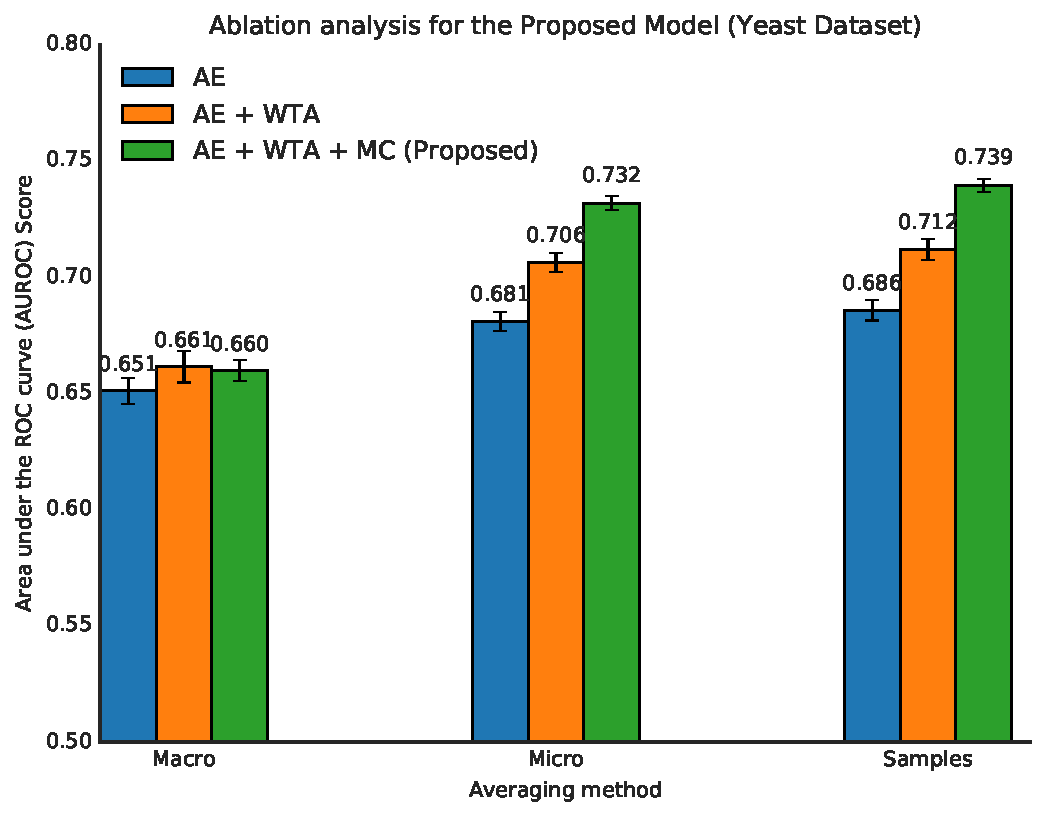
\includegraphics[width=\textwidth]{ch04/ab/ab_yeast}
        \caption{Yeast}
        \label{results:fi_yeast_base}
    \end{subfigure}
    ~ %add desired spacing between images, e. g. ~, \quad, \qquad, \hfill etc. 
      %(or a blank line to force the subfigure onto a new line)
    \begin{subfigure}[b]{0.45\textwidth}
        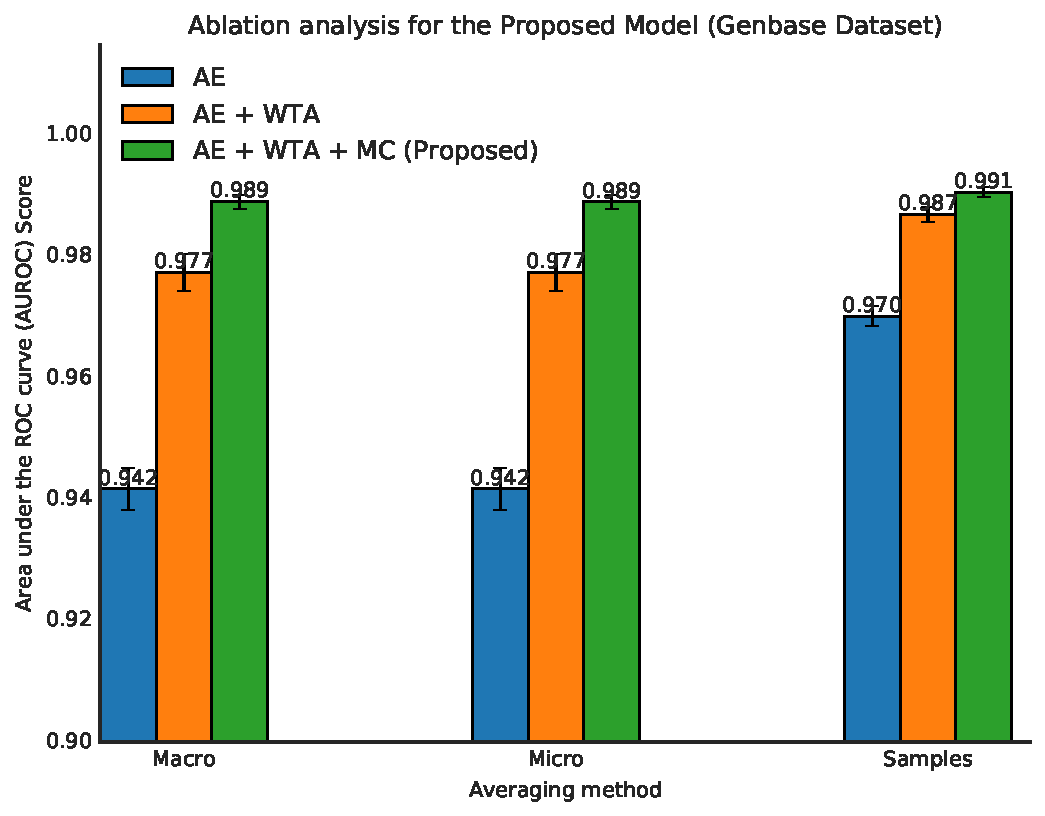
\includegraphics[width=\textwidth]{ch04/ab/ab_genbase}
        \caption{Genbase}
        \label{results:fi_genbase_base}
    \end{subfigure}
    \caption{Ablation analysis for both datasets}
    \label{results:ab_analysis}
\end{figure}

\chapter{Conclusion}
\label{Conclusion}


\section{Future work}
\label{FutureWork}


%------------------------------------------------------------------------------
%	THESIS CONTENT - APPENDICES
%------------------------------------------------------------------------------

\appendix % Cue to tell LaTeX that the following "chapters" are Appendices

% Include the appendices of the thesis as separate files from the Appendices folder
% Uncomment the lines as you write the Appendices

% \include{Appendices/AppendixA}
%\include{Appendices/AppendixB}
%\include{Appendices/AppendixC}

%------------------------------------------------------------------------------
%	BIBLIOGRAPHY
%------------------------------------------------------------------------------

\printbibliography[heading=bibintoc]

%------------------------------------------------------------------------------

\end{document}  
